\documentclass[11pt]{article}
%fartboner420
\newpage
\clearpage
\usepackage{geometry} % sets more standardized margins
\geometry{letterpaper,
left=1.5in,
right=1in,
top=1in,
bottom=1in}
\usepackage{tikz}
\usepackage{graphicx}
\usetikzlibrary{calc} % some graphics functions I use 
\graphicspath{{figures/}}
\usepackage{abstract} % abstract function
\usepackage{mathtools}
\usepackage{float}
\usepackage{pdfpages}
\usepackage{verbatim}
\usepackage{array}
\usepackage{soul}
\usepackage{setspace}
\usepackage{color}
\usepackage[utf8]{inputenc}
\usepackage[english]{babel}
\usepackage{longtable}
\usepackage{multirow}
\usepackage{booktabs}
\usepackage{textcomp}
\usepackage{gensymb}
\usepackage{setspace}
\usepackage{hyperref}    % make hyperlinks for easy navigation
\hypersetup{colorlinks=true,linkcolor=black,citecolor=black,urlcolor=blue}  % allows for highlighting
\usepackage{titlesec}

\setcounter{secnumdepth}{4}
\setcounter{tocdepth}{4}

\titleformat{\paragraph}
{\normalfont\normalsize\bfseries}{\theparagraph}{1em}{}
\titlespacing*{\paragraph}
{0pt}{3.25ex plus 1ex minus .2ex}{1.5ex plus .2ex}

\newcommand{\n}{\par}
\newcommand{\p}{\par\hspace{1em}}

\renewcommand{\absnamepos}{flushleft} % left justifies abstract
\setlength{\absleftindent}{0pt}
\setlength{\absrightindent}{0pt}
\newcolumntype{L}{>{\centering\arraybackslash}m{12cm}}

\linespread{1.3}

\setlength{\parskip}{1em} % sets space between paragraphs
\setlength{\parindent}{0em} % Left justifies paragraphs after a \par command 
%\usepackage{nopageno}

\begin{document}

\pagenumbering{gobble}
\title{ \textbf{Tachometer for Sheaff's Buddy's Boat}}
\author{Colin Leary, EE \\ Chris Martin, CE}
\date{\today\\[2ex]%
University of Maine\\%
ECE403 Final Report}
\maketitle
\newpage
\clearpage

\pagenumbering{roman}
\begin{abstract}
The design of the Tachometer for Sheaff's Buddy's Boat (TFSBB), a tachometer for a Celebrity Champion power boat, is described. A tachometer is a device that shows how fast an engine is turning. Most tachometers simply display the engine speed, however the TFSBB also reads sensors from a gasoline engine and displays the results to a  detachable LCD display. The TFSBB met all specifications with a 5V DC-DC power supply and detachable display capable of showing engine revolutions per minute, engine temperature and oil pressure, and battery voltage. Primarily, the TFSBB drove an analog gauge to an accuracy of within 100 revolutions per minute.

\end{abstract}
\newpage
\clearpage

\begin{singlespacing}
    \tableofcontents
    \newpage
    \clearpage
    
    \listoffigures
    \newpage
    \clearpage
    
    %\listoftables
    %\newpage
    %\clearpage
\end{singlespacing}

\section{Introduction}
\label{sec:intro}
\pagenumbering{arabic}
This report describes the design and construction of the Tachometer for Sheaff's Buddy's Boat (TFSBB), a replacement tachometer driver for a 1988 Celebrity Champion power boat. A tachometer is a device that measures the speed an engine is turning, typically measured in revolutions per minute (RPM).  The power boat, belonging to Stewart Harvey, has an analog gauge and failed analog driver circuitry. The tachometer being described in this report is intended to replace the failed circuitry.

The TFSBB is designed to work with a four cylinder, four stroke, gasoline engine. In a gasoline engine, the ignition coil connects to a distributor that provides spark to the individual spark plugs. Because each cylinder fires every other rotation, the coil fires twice per revolution on a four cylinder engine. Thus, the RPM of the engine can be determined by measuring the frequency of the ignition signal from the engine. %Due to the four cylinders of the engine, the RPM of the motor is half of the number of pulses measured on the ignition signal. The same concept can be applied to other engines that employ similar ignition techniques.


When it comes to similar products, there is no equivalent on the market. Most tachometers come pre-installed by the vehicle manufacturer, and are integrated into the vehicle. One can buy a stand-alone tachometer unit, which contains both the gauge and driver circuitry, or can buy ICs that convert frequency to a voltage. The TFSBB however, fills a gap in the market, being a custom replacement for broken tachometer driver circuitry. The TFSBB also uses a microcontroller to accomplish the task of additional functionality such as measuring oil pressure and temperature.

An additional feature of the tachometer is a detachable liquid crystal display (LCD) showing analog engine information such as temperature, pressure, and battery voltage. Additional engine information alerts the operator to potential engine problems. The specifications for the tachometer are given below and are extracted from the project contract found in Appendix~\ref{app:contract}.

The project specifications include a DC-DC converter to step the nominal 12V battery voltage down to 3.3V. The DC-DC converter must output within 5\% of the specified voltage with less than 100mV of ripple. The tachometer must also be able to drive the gauge needle between 1000RPM and 4000RPM with an accuracy of 100RPM. The project must be built on a printed circuit board (PCB), be a deliverable product, and be capable of showing the RPM, coolant temperature, oil pressure, and battery voltage. The DC-DC converter specification was altered during the design process to supply 5V instead of 3.3V. The voltage change is discussed in Section~\ref{sec:ps}. The chosen method for displaying coolant temperature, oil pressure, and battery voltage is an LCD.

Section~\ref{sec:break} includes a functional block diagram and discusses the high level operation of the blocks. Section~\ref{sec:det} delves into the design process and decisions in more detail. Section~\ref{sec:res} reviews the results of the tachometer and presents evidence to prove functionality. Finally, Section~\ref{sec:con} concludes the report with a brief discussion of the results and a review of the report.


\section{Breakdown}
\label{sec:break}
This section gives a high-level overview of the functional blocks of the tachometer. Figure~\ref{fig:block} shows the tachometer block diagram.


\begin{figure}[H]
    \centering
    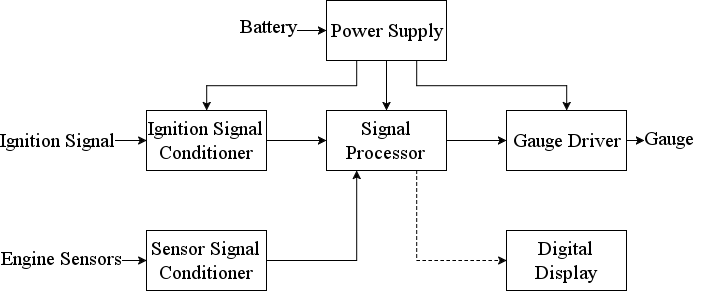
\includegraphics[width=\textwidth]{blocks}
    \caption{Tachometer block diagram}
    \label{fig:block}
\end{figure}

The system works as follows: the power supply is a switching DC-DC converter that steps the nominal 12V of the battery down to a regulated 5V to power the project. Additionally, a linear DC-DC converter steps the battery voltage down to 10V for the gauge driver circuitry, discussed later. The ignition signal conditioner block filters the ignition signal to produce a 0V to 5V square wave for the signal processor. The ignition signal conditioner protects the rest of the system from the high voltages of the ignition system. The sensor signal conditioner steps 12V signals from the temperature, pressure, and voltage sensors down to 5V signals. Signals from the the ignition and sensor conditioners go to the signal processor, which is responsible for controlling the gauge driver and digital display. The gauge driver amplifies the signal from the signal processor to drive the gauge to the proper position. The signal processor can be calibrated upon installation, allowing the tachometer to be adjusted to gauge variations. The digital display is a detachable LCD screen which is capable of displaying the engine RPM as well as the other specified inputs.


\subsection{Power Supply}
The power supply, a switching DC-DC converter, steps the 12V battery voltage down to 5V positive voltage rail of the tachometer. A switching DC-DC converter is more efficient than a linear regulator and thus dissipates less heat. The DC-DC converter uses a TI simple switcher integrated circuit, which simplifies the design and construction process. Using a simple switcher means no need to select a transistor or design a bootstrap circuit, a complicated process with a conventional DC-DC converter. It also has a built in feedback network, which is able to compensate for variations in the input voltage. 


\subsection{Ignition Signal Conditioner}
The ignition signal conditioner (ISC) converts the ignition signal from the engine into a digital signal for the signal processor. As the ignition signal is generated by the engine's ignition coil, a significant amount of electrical noise is present with the signal. Voltage spikes in excess of 100V are also present, which would damage the signal processor if not properly handled. To protect the rest of the tachometer circuitry from these voltage spikes, the ISC must prevent the ignition signal from exceeding the positive rail voltage or dipping below the reference rail voltage (0V).

To increase the signal processor's ability to reliably measure the ignition signal frequency, the ISC must also filter out the high frequency noise caused by the ignition coil. A low pass filter, operational amplifier buffer, and a comparator accomplish the task of generating a low-noise square wave which is then fed to the signal processor.

\subsection{Gauge Driver}

The gauge driver runs the physical tachometer gauge. The gauge operates by controlling the voltages on the three input wires to change the magnetic field in the gauge. The gauge driver amplifies the signal from the signal processor to drive the gauge.

\subsection{Sensor Signal Conditioner}

The sensors in the engine operate on the logic level of the battery ($\sim$12V). To allow the signal processor to measure the sensor signals, they must first be reduced to a 5V logic level. The engine sensors consist of heat-varying, and pressure controlled resistors for engine temperature and oil pressure, respectively. The gauges in the dashboard of the boat drive a current through the resistive sensors and measure their voltages. So as not to affect the sensor readings with the measurement circuitry, the signal conditioner uses a high input impedance resistive voltage divider followed by an operational amplifier unity gain buffer. The output of this stage is a 0V to 5V direct current signal.

\subsection{Digital Display}

The digital display lets the user see a readout of the engine RPM and engine sensors. The display can safely be hot swapped when the tachometer is in operation. When the display is connected, a signal is sent to the signal processor to indicate its presence. The display is then initialized to output engine sensor information.

\subsection{Signal Processor}
The signal processor takes input signals and produces output signals that ultimately become human readable. First, the signal processor receives the conditioned tachometer signal and calculates its frequency. An algorithm finds engine RPM from the input and produces an output signal to run the gauge driver.

Next, an analog to digital converter (ADC) converts the engine sensor inputs to a digital value. An ADC calibration algorithm converts these input values into output values for pressure, temperature, and battery voltage. Finally the signal processor sends the engine RPM and human readable sensor information to the digital display and gauge driver.

\section{Details}
\label{sec:det}
With the high level function of the tachometer components explained, this section describes the hardware and software design process of the tachometer. 

\subsection{Hardware}
Before delving into the software controlling the tachometer or the methods and algorithms, the hardware must first be presented to give context to the software design. This order of presentation is not perfect, as many hardware design decisions were influenced by the presence of the signal processor and its selection of peripherals. A complete schematic is given in Appendix~\ref{app:schem}. The schematic is too large to fit on a single page and remain readable, so it is broken into four separate pages. Figure~\ref{fig:block_schem} serves to illustrate the connection between the different pages of the schematic.

\begin{figure}[H]
    \centering
    \includegraphics[width=.8\textwidth]{schem_block}
    \caption{Diagram of schematic page relationship}
    \label{fig:block_schem}
\end{figure}

The power supply and sensor conditioner are built on separate PCBs from the tachometer, as they are required to meet specifications, but not essential to operation of the tachometer's primary function - measuring RPM. While a power supply must be present in order for the tachometer to function, the designed power supply is not a requirement. The power supply could be replaced with an off-the-shelf switching  or linear regulator, such as the LM7805.

\subsubsection{Power Supply}
\label{sec:ps}
The power supply is a DC-DC converter that reduces the nominal 12V of the battery to a stable 5V for the tachometer. Presented is a justification of the output voltage choice and engineering decisions behind component selection.

\paragraph{Output Voltage}
The initial specified output voltage of the power supply was 3.3V, however during the design process it was determined a higher voltage of 5V would improve performance when driving the gauge. As is discussed in detail in Section~\ref{sec:gauge}, the gauge is controlled by driving current through the coils in a specific manner. In order to drive enough current through the gauge coil, a large enough rail voltage must be present for the gauge driver circuitry. 

Since the gauge of the customer's boat is not removable from the boat and unavailable for testing, measurements were taken to characterize the gauge and a similar gauge was used for testing purposes. The boat gauge had a measured impedance of 230$\Omega$ and the test gauge had a measured impedance of 80$\Omega$. The low impedance test gauge was able to be driven reliably with the lower rail voltage of 3.3V. However, the higher impedance gauge on the boat results in a coil current of only 14mA at maximum differential. A low coil current in the gauge risks unreliable performance. For this reason, the rail voltage was increased to ensure reliable operation.

To comply with contract specifications, the designed power supply was made to be adjustable to either 3.3V or 5V, and the tachometer was designed to operate at both voltage levels. The tachometer is recommended to be run at the higher 5V.

\paragraph{Design}
A DC-DC converter was built to reduce the 12V battery to 5V for the tachometer circuitry. The DC-DC converter was designed with the Texas Instruments LM2675 Simple Switcher. A simple switcher was used for a few reasons: simplicity to construct, documentation and parts availability, and the built-in feedback to ensure stable output voltage. Shown below in Figure~\ref{fig:lm2675_ps} is the generic schematic as suggested by the datasheet. 

\begin{figure}[H]
    \centering
    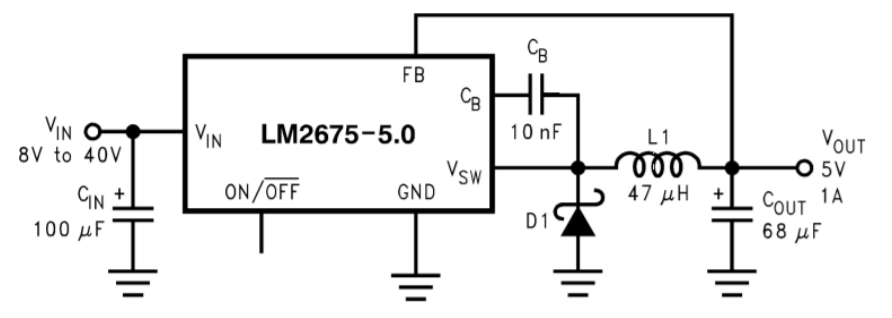
\includegraphics[width=.75\textwidth]{lm2675_schem}
    \caption{Power supply schematic from datasheet~\cite{lm2675}}
    \label{fig:lm2675_ps}
\end{figure}

The suggested schematic is for a 5V output DC-DC converter. During the prototyping process, a 100uH inductor value was selected for availability reasons. Calculations indicate that a minimum inductor value would be 47uH. The minimum inductor value is rarely an ideal choice, as manufacturing variations could result in the DC-DC converter failing to remain in continuous current mode. The inductor stores energy, acting as a current source for the output when the switcher is "off". If the inductor cannot store enough charge, the DC-DC converter may not be able to supply enough current and the output voltage will fluctuate. The inductor selection chart from the LM2675 datasheet is shown below in Figure~\ref{fig:inductor}.

\begin{figure}[H]
    \centering
    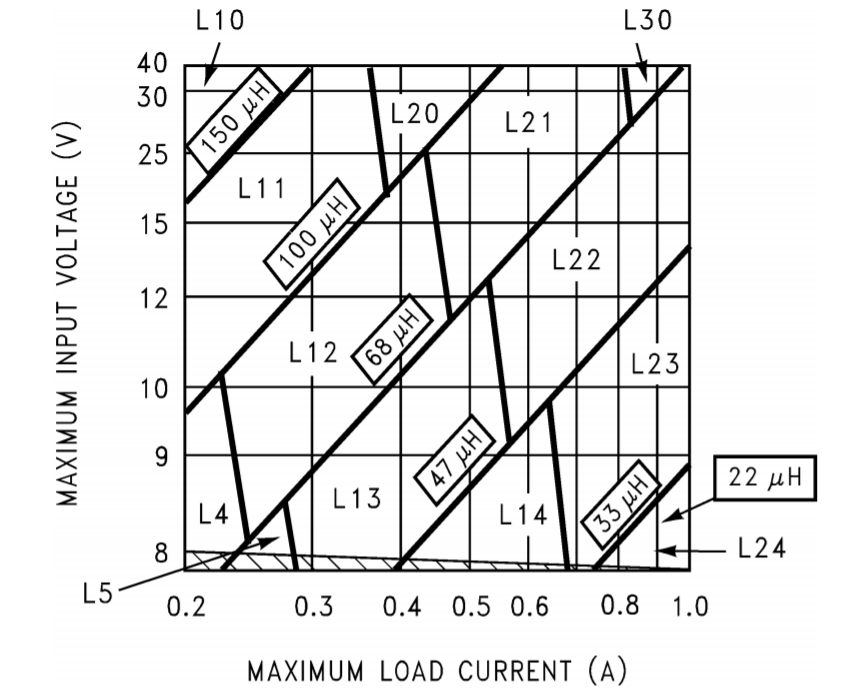
\includegraphics[width=.52\textwidth]{ps_ind}
    \caption{TI simple switcher inductor selection chart~\cite{lm2675}}
    \label{fig:inductor}
\end{figure}

The chart is specifically intended for 5V implementations of the LM2675. Similar charts are present for other voltage levels. Despite datasheet tables and current ripple calculations suggesting the use of a 68uH inductor, the 100uH was used in the final design. A slightly higher inductor value than is recommended typically does not negatively impact power supply performance. The inductor stores energy while the switcher is on, and then dumps that energy when the switcher is off. For this reason, a larger inductor allows more current to be drawn, without risking discontinuous operation. As per datasheet recommendation, a low equivalent series resistance (ESR), 100uF capacitor was added to the input node of the power supply to reduce transients into the converter. The Schottkey diode, D1 in Figure~\ref{fig:lm2675_ps}, needed to be capable of switching quickly in order to keep up with the Simple Switcher's internal frequency of 260kHz. It is also important to use a Schottkey diode due to their low forward voltage drop. This low drop allows the diode to turn on sooner, creating a more stable DC output.

Output capacitors were also needed to smooth out the ripple created by the switching of the LM2675 chip. Similarly to inductor selection, the datasheet had charts to aid in the determination of output capacitor values. The output capacitors were selected to be low ESR ceramic capacitors. When designing the PCB, space for five capacitors was allocated for each decade ranging from 100uF down to 10nF to ensure output ripple could be kept below the specified 100mV. Each decade of capacitor filters a different frequency range, thus implementing more decades allows for better overall filtering.

To make the output adjustable, the LM2675-ADJ was used along with a potentiometer based resistor network on the feedback line. Figure~\ref{fig:feedback} below shows the recommended LM2675-ADJ with feedback network.

\begin{figure}[H]
    \centering
    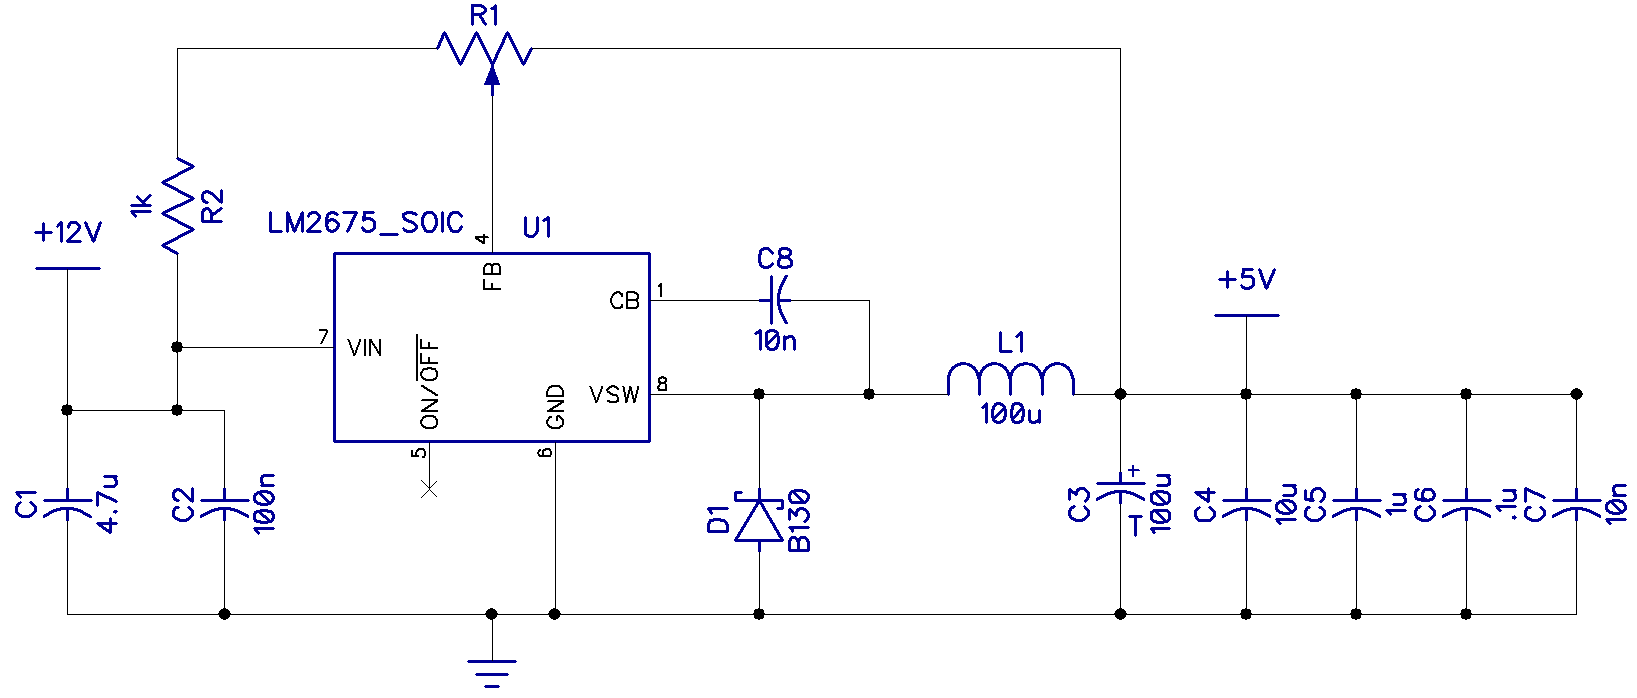
\includegraphics[width=\textwidth]{ps}
    \caption{Adjustible power supply with feedback network}
    \label{fig:feedback}
\end{figure}

The position of the potentiometer, R1, in the schematic determines the output voltage of the regulator. By adjusting the potentiometer, the output voltage can be adjusted as needed.

\subsubsection{Ignition Signal Conditioner}
The ignition signal conditioner was one of the primary challenges presented by this project. The ignition system of the engine employs a coil to gather charge, which is then dissipated to make the spark plug ignite the fuel in the engine cylinder. The process of building and releasing charge produces a noisy ignition signal that needs to be measured by the tachometer to determine engine RPM. The ISC filters out the noise and prevents large magnitude transients from destroying the tachometer circuitry. If the tachometer is not sufficiently protected against noise and large magnitude transients, the system would not work reliably.

\paragraph{Ignition System} %%%%%%%%%%%%%%%%%%%%%%% IGNITION
\label{par:ignition}

The ignition system on a gasoline engine fires the spark plugs to make the engine run. Figure~\ref{fig:ignition} shows the ignition system typically used on older gasoline engines, such as that used in the 1988 Celebrity Champion.



\begin{figure}[H]
    \centering
    \includegraphics[width=\textwidth]{ignition}
    \caption{Engine ignition system}
    \label{fig:ignition}
\end{figure}

When the ignition switch is turned on, the positive side of the ignition coil is connected to 12V. A distributor is the device on an engine that contains the points and fires the spark plugs at the correct time. As the distributor turns, the points close. Closing of the points connects the negative side of the ignition coil to ground causing current to flow though the coil. When current flows through the coil, a magnetic field is built up inside the windings. As the distributor keeps turning, the points open again, releasing the magnetic field in the form of high voltage to the spark plugs. The condenser, or capacitor, keeps voltage from arcing across the contacts of the points. Figure~\ref{fig:boat_noise} illustrates one of the biggest challenges of hardware design in this project: voltage spikes.

\begin{figure}[H]
    \centering
    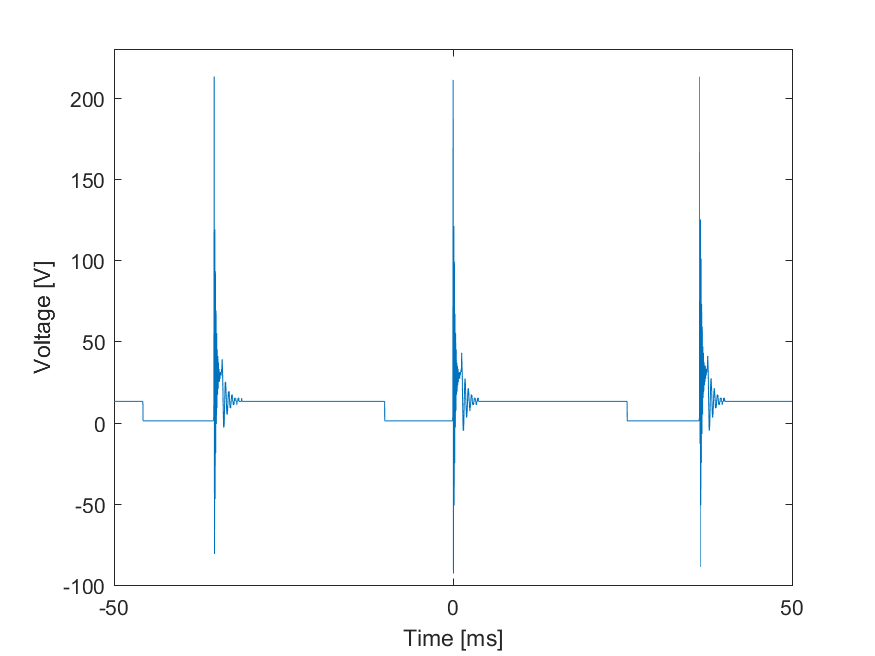
\includegraphics[width=.8\textwidth]{boat_raw}
    \caption{Ignition signal from Celebrity Champion}
    \label{fig:boat_noise}
\end{figure}

 The signal processing unit can only tolerate a 5V signal, however, when high voltages are created using a coil of wire, large voltage spikes and high amounts of noise are created. As shown in Figure~\ref{fig:boat_noise}, these voltage spikes can be in excess of 200V.

\paragraph{Design}
The signal shown in Figure~\ref{fig:boat_noise}, needs to have the voltage spikes removed. It is crucial that this be done in a robust manner to ensure long-term reliability of the tachometer. The bulk of this task can be handled by a few passive components. First, a resistive voltage divider reduces the logic level from 12V to 5V. A pair of diodes clamps the signal, preventing it from exceeding the positive rail voltage or dipping below the reference rail voltage. The resistive voltage divider also acts as a current limit, protecting the diodes from damage. Finally, a capacitor creates a low pass filter. This partial circuit is shown below in Figure~\ref{fig:clamp_filter}.

\begin{figure}[H]
    \centering
    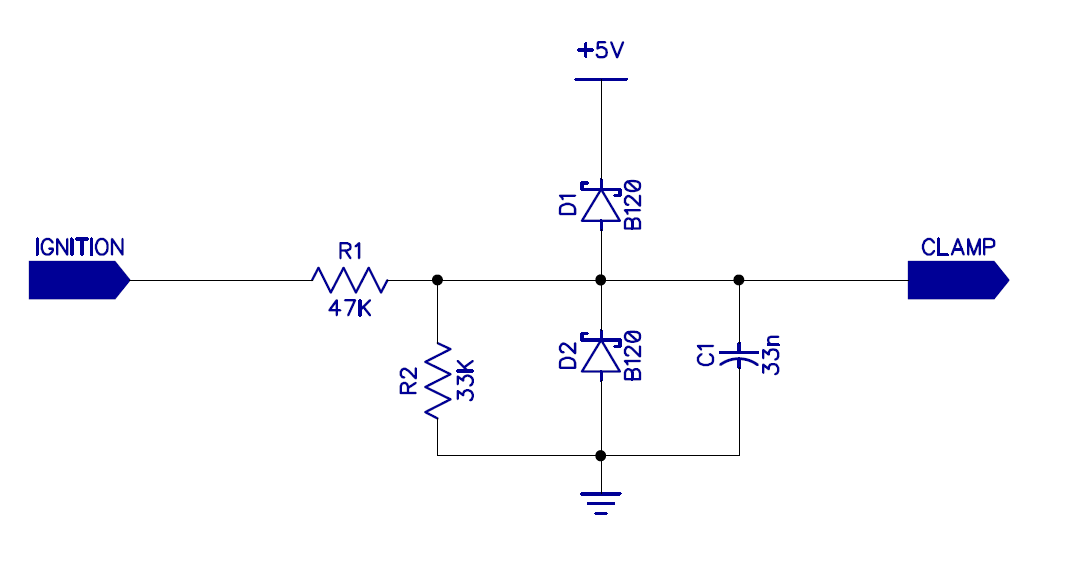
\includegraphics[width=.85\textwidth]{clamp}
    \caption{Partial input filter circuit}
    \label{fig:clamp_filter}
\end{figure}

The resistor values were chosen such that they created a voltage divider with a ratio of approximately $5/12$ and had a total resistance over 50k$\Omega$. The voltage divider current limits the signal while stepping down the logic level. To effectively clamp the signal to the supply voltage, fast switching, low voltage drop diodes were needed. Low voltage drop was needed to allow the signal to be clamped to a voltage close to that of the supply. Fast switching was needed to change state at a speed which matches that of the high frequency noise. Schottkey diodes have all of these characteristics. The capacitor selection process involved calculating the maximum frequency the ignition signal could reasonably reach and then placing the cutoff frequency of the low pass filter slightly above that.

The maximum frequency of the ignition signal is 300Hz (corresponding to 9000 engine RPM). With a maximum input frequency of 300Hz, a cutoff frequency above 1kHz does not cause interference with the ignition signal integrity. The low pass filter created by R1, R2, and C1 places a cutoff frequency around 1.56kHz.

Figure~\ref{fig:diode} shows the ignition signal after passing through the partial conditioning circuit.
\begin{figure}[H]
    \centering
    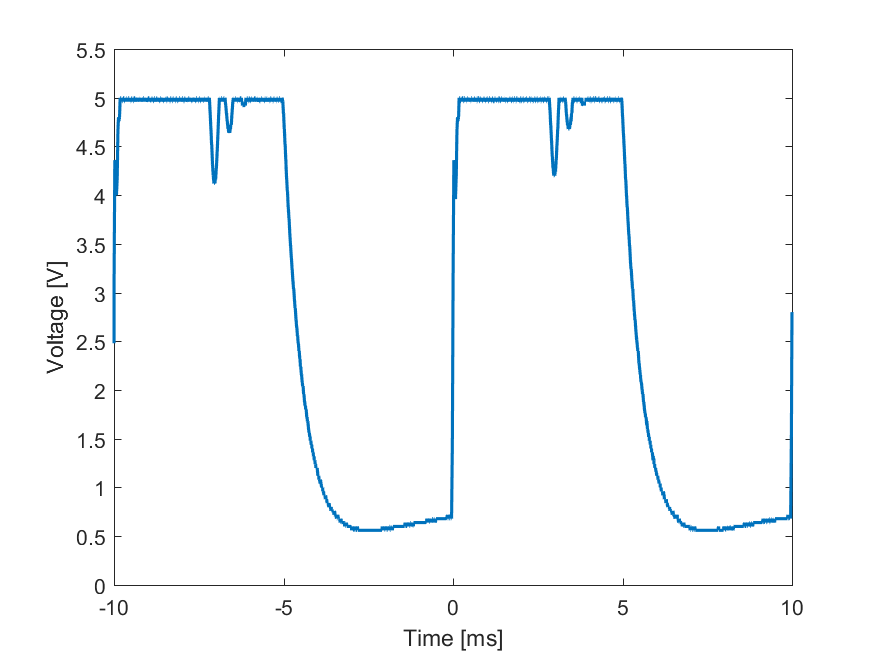
\includegraphics[width=.75\textwidth]{diode}
    \caption{Ignition signal after clamping and filtering}
    \label{fig:diode}
\end{figure}

Most noise is removed, and the output resembles a square wave. To further condition the signal, it was fed into a comparator to generate a clean square wave for the signal processor. To increase reliability, the comparator was configured to use hysteresis. Since configuring hysteresis lowers the input impedance of the comparator, the output of the clamp was passed through an operational amplifier unity gain buffer before being passed to the comparator. The additional ignition conditioning circuitry is shown in Figure~\ref{fig:comp} below.

\begin{figure}[H]
    \centering
    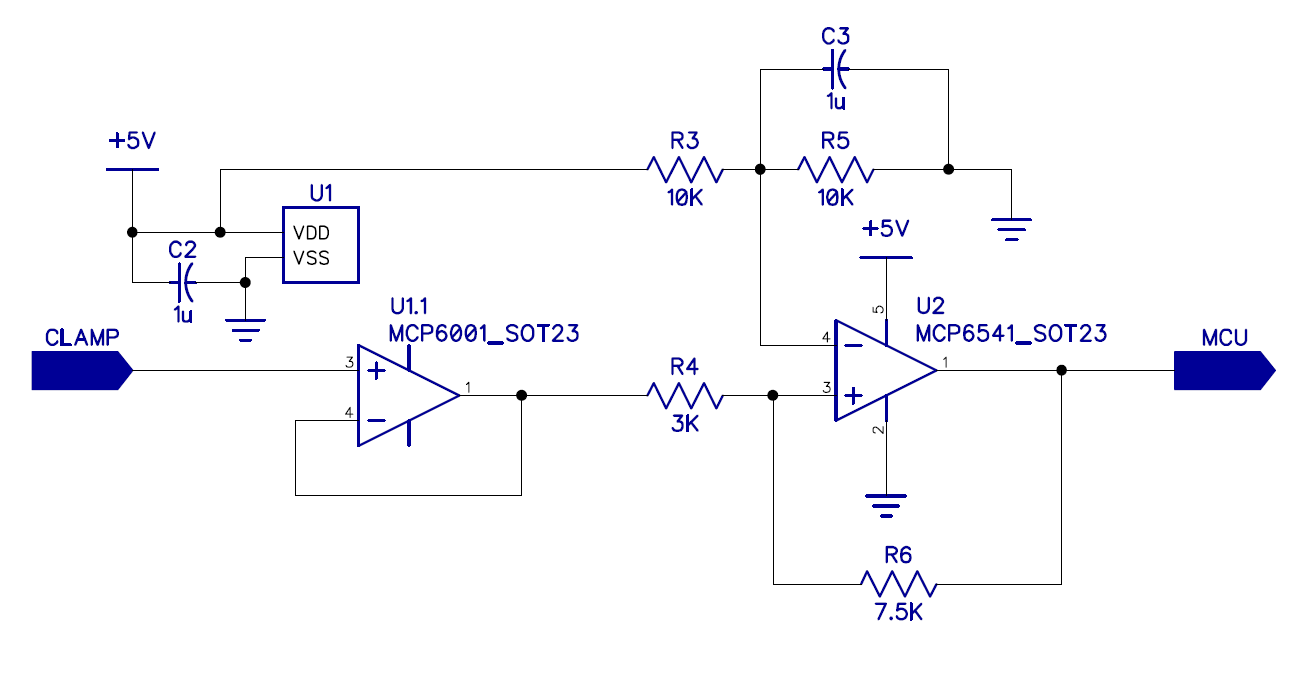
\includegraphics[width=.9\textwidth]{comp}
    \caption{Ignition signal current buffer and comparator}
    \label{fig:comp}
\end{figure}

To determine the resistor values to set the hysteresis of the comparator,  Equations~\ref{eq:hist1}~and~\ref{eq:hist2} were adapted from the datasheet\cite{mcp6541} for this application.

\begin{equation}
\label{eq:hist1}
    V_{TLH} = 2.5V(1+\frac{R_4}{R_6}) - V_{OL}(\frac{R_4}{R_6})
\end{equation}
\begin{equation}
\label{eq:hist2}
    V_{THL} = 2.5V(1+\frac{R_4}{R_6}) - V_{OH}(\frac{R_4}{R_6})
\end{equation}

In the equations above, $V_{OH}$ and $V_{OL}$ are the desired high and low output voltages, respectively. $V_{THL}$ and $V_{TLH}$ are the input voltages at which the output will change from high to low, or low to high, respectively. Using the equations above, the resistor values were determined such that an input voltage of 3.5V or more will cause the comparator to switch output from low to high, and an input voltage of 1.5V or less will cause the comparator to switch from high to low. The output of the comparator is shown below in Figure~\ref{fig:conditioned}.

\begin{figure}[H]
    \centering
    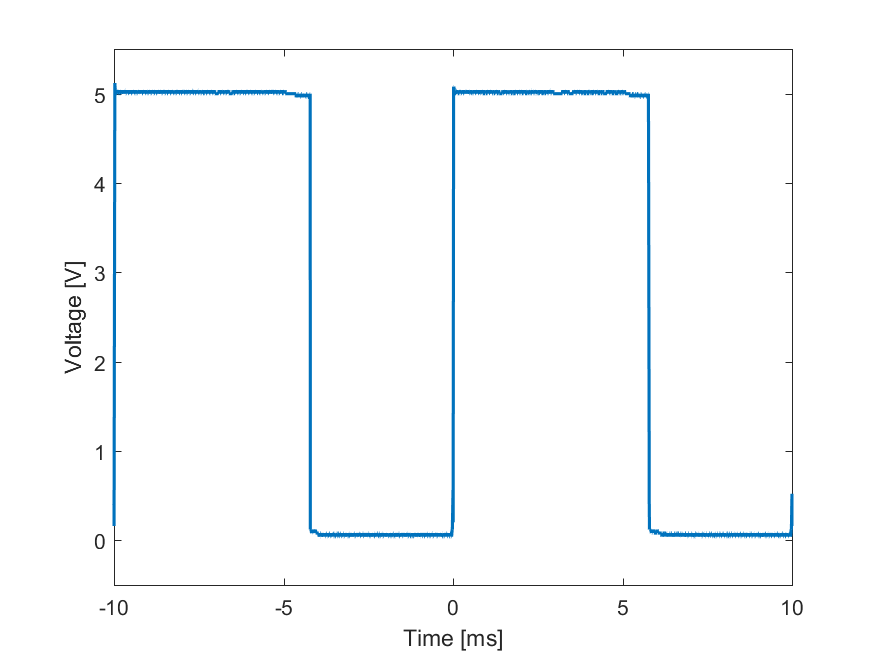
\includegraphics[width=.7\textwidth]{conditioned}
    \caption{Conditioned ignition signal}
    \label{fig:conditioned}
\end{figure}

With the ignition signal conditioned to a square wave, the signal processor can now accurately measure the frequency with a digital pin. The filtering and and buffering done by the ignition signal conditioner also protects the rest of the circuit from the noise introduced by the ignition signal.

\subsubsection{Gauge Driver} %%%%%%%%%%%%%%%%%%%%%%%%%%%%%%%%%%%%%%%%%%% Gauge Driver %%%%%%%%%%%%%%%%%%%%%%%%%%%%%%%%%%%
\label{sec:gauge} % label to gauge driver for reference elsewhere 
The analog tachometer gauge on the Celebrity Champion is an air core gauge. This section provides discussion on how an air core gauge works, and how a hardware driver was built.
\paragraph{Air Core Gauge}
The air core gauge has three input wires, one at a reference voltage, and two at voltages above and below the reference.

Figure~\ref{fig:aircore} shows a representation of an air core gauge from the LM1819 datasheet.


\begin{figure}[H]
    \centering
    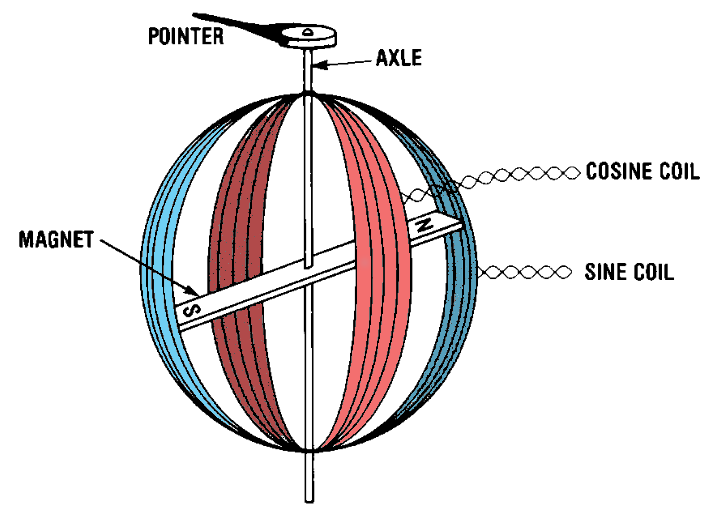
\includegraphics[width=.75\textwidth]{aircore}
    \caption{Diagram of air core gauge~ \cite{lm1819}}
    \label{fig:aircore}
\end{figure}

The air core gauge consists of a magnet and two coils of wire. The pointer is connected to a magnet that lies between the two coils of wire that are 180$^{\circ}$ degrees apart. When a voltage is applied to the coils, a magnetic field is created that moves the magnet, and in turn the pointer. Figure~\ref{fig:tach} shows the relationship between input voltage and pointer deflection.

\begin{figure}[H]
    \centering
    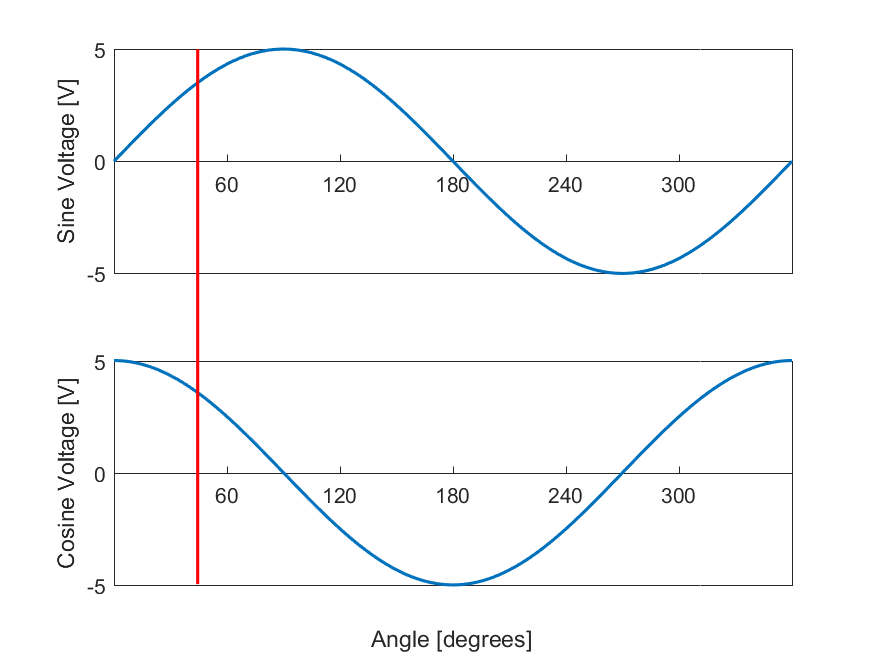
\includegraphics[width=.8\textwidth]{sincos}
    \caption{Input waveform to gauge}
    \label{fig:tach}
\end{figure}

The zero degree line is where both differential inputs to the gauge are at the same voltage and thus the pointer is at zero degrees of deflection. As long as the sine and cosine coils follow the voltage relationship shown in Figure~\ref{fig:tach}, the pointer turns smoothly in a circle.
\paragraph{Design}
Due to the impedance of the coils in the gauge on the Celebrity Champion, the reference voltage was chosen to be 5V and the rail voltage was 10V. This was done so that the peak current flowing through the coils was around 22mA. If the 3.3V logic level was used, a peak current of only about 14mA would flow through the coils. Testing showed that a peak current of less than 10mA was not sufficient for reliable gauge operation, and the 14mA of the 3.3V logic level was too close to this lower limit. Since reliability is a large concern for this project, a higher logic level was used.

Since the output from the signal processor is only 5V, a buffering level shifter was built. The cosine coil driver is shown in Figure~\ref{fig:buflevel}, an identical one was also built for the sine coil. 

\begin{figure}[H]
    \centering
    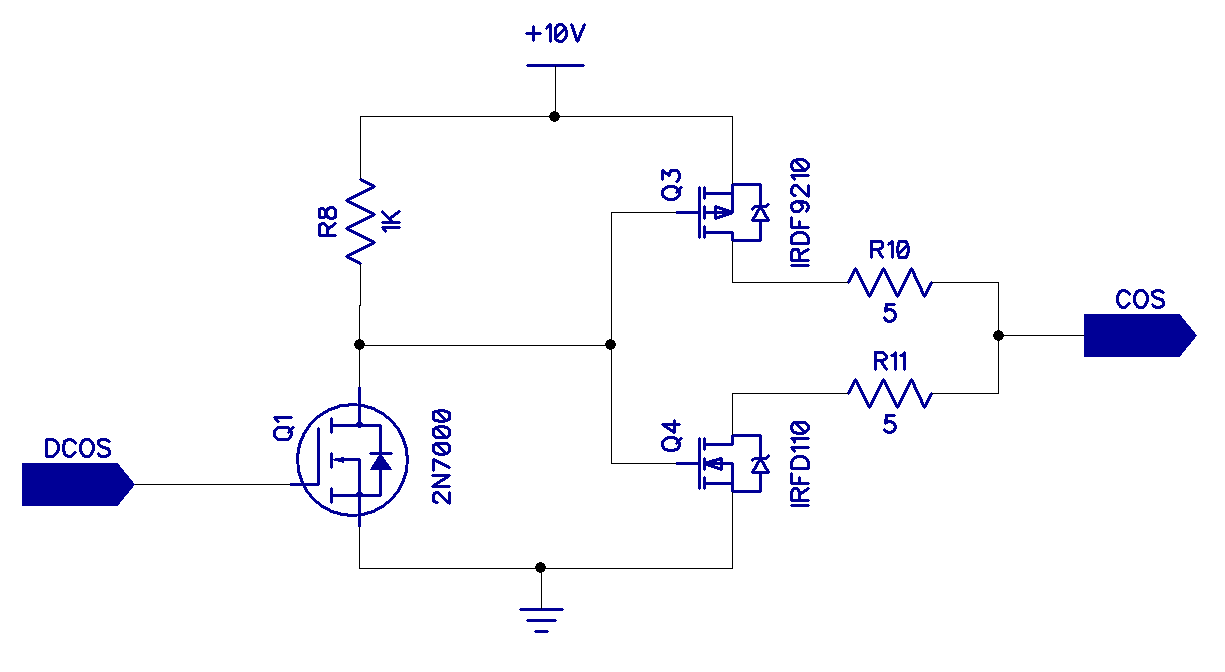
\includegraphics[width=\textwidth]{gauge_driver}
    \caption{Buffering level shifter to drive tachometer}
    \label{fig:buflevel}
\end{figure}


A 0V input to DCOS on the level shifter creates an output of 0V, and an input of 5V creates an output of 10V. The result is a 5V center voltage to the tachometer with a 0V to 10V on the differential inputs of the air core gauge.

%%%%%%%%%%%%%%%%%% SOFTWARE STUFF HERE
\subsection{Software}
This section discusses the software running on the signal processor.
The main loop checks for new raw input values and converts them human readable information. New input values include: ADC values from engine sensors, RPM values from the ignition signal, and request for programming mode. After processing the inputs, the main loop outputs the values to either the Gauge Driver, or the detachable display. Figure~\ref{fig:softbd} shows the software block diagram.
\begin{figure}[H]
    \centering
    \includegraphics[width=.75\textwidth]{softBD}
    \caption{Software block diagram of Signal Processor}
    \label{fig:softbd}
\end{figure}

The software block diagram helps understand how the signal processor works. The interrupts set flags that the main loop checks for each time around. If a flag is set, the main loop performs a certain task. For example, when the ignition input interrupt is triggered, an algorithm is run to determine the frequency of the input signal. The input frequency is then converted into an RPM value to be sent to the gauge driver or the digital display.

\subsubsection{Programming Mode} %%%%%%%%%%%%%%%%%% PROGRAMMING MODE
Programming mode is for calibrating the tachometer for a particular installation. A couple parameters need to be set: the range of the analog gauge, and the analog input values for the engine sensors. A serial interrupt alerts the main loop if a user has requested programming mode. After calibration has been performed, the calibration values are stored to a data structure in the electronically erasable programmable read only memory.

\subsubsection{ADC} %%%%%%%%%%%%%%%%%% ADC
The engine sensors connect to the ADC inputs on the microcontroller. The ADC produces values between 0 and 1023, the ADC routine then converts these into human readable information. First, the main loop requests an ADC reading for a certain sensor input. Once a request is made, the ADC interrupt is turned on. After the ADC value is recorded, the ADC interrupt triggers the ADC calculation, which then converts the input to a human readable information using the values stored in the configuration structure.


\subsubsection{Conditioned Ignition Input} %%%%%%%%%%%%%%%%%% TACH INPUT
To calculate the engine RPM, the conditioned ignition input is connected to a hardware interrupt pin on the microcontroller. Every time a rising edge is detected on the input, the conditioned ignition interrupt is triggered. When the interrupt is triggered, it reads the value of Timer~1. The microcontroller runs at 8MHz, and timer~1 is configured with a divide by 8 prescaler, meaning timer~1 is counting  microseconds. The input interrupt saves the value of timer~1 to a global variable and resets the timer.

The RPM calculation block then looks at the value of the timer and uses that value to calculate the input frequency of the ignition input, which can then be correlated to the engine RPM. Since timer~1 is a 16-bit timer, the slowest input period that can be calculated in 65535 microseconds, or about 15Hz. If the input frequency is lower than 15Hz, Timer~1 overflow interrupt is triggered and alerts the RPM calculation block allowing frequencies with a period as high as 65535 + 65535 = 131072 microseconds, or 7.6Hz to be calculated. With a speed that low, the engine is assumed to be stopped, and the output RPM signal is set to zero.

After determining the input frequency, the RPM calculation block needs to convert frequency to RPM. Equation~\ref{eqn:RPM} shows the calculation for a four cylinder, for stroke engine.
\begin{equation}
    \label{eqn:RPM}
    RPM = 30*Hz
\end{equation}
After the RPM is calculated, the value is saved to be processed by the gauge driver.

\subsubsection{Gauge Output} %%%%%%%%%%%%%%%%%% TACH OUTPUT
The gauge output driver must interface with the hardware output driver described in Section~\ref{sec:gauge}. Since the microcontroller used in this project does not have a digital to analog converter, it uses pulse width modulation (PWM) to simulate an analog voltage with a pulsed square wave. A 31kHz PWM frequency was used in this project because it is higher than human hearing, thus avoiding a high pitch humming from the air core gauge.

Section~\ref{sec:gauge} discussed driving the gauge with two sine waves, however the gauge driver software only changes the value of one input at a time. Figure~\ref{fig:scPWM} shows the curve used in software.

\begin{figure}[H]
    \centering
    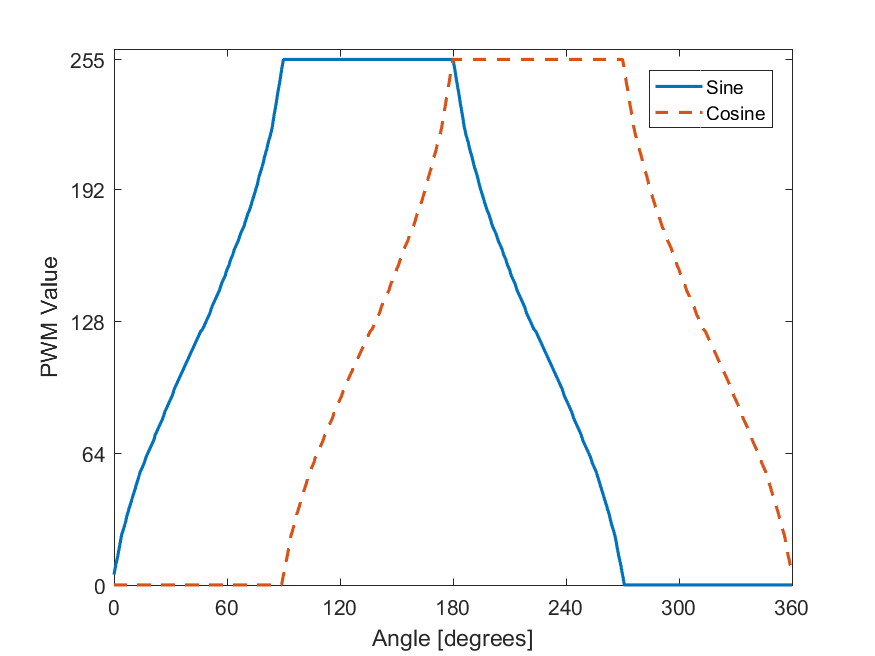
\includegraphics[width=\textwidth]{sinarr}
    \caption{Sine and cosine curve used for gauge driver}
    \label{fig:scPWM}
\end{figure}

As discussed before, the pointer on the gauge still moves linearly, however the driver uses a lookup table with a tangent curve. The result is that one output, either sine or cosine, is always either high or low, and the other input changes with pointer deflection angle. This method of gauge control was easier and faster to design in software than changing both inputs at the same time.

\subsubsection{Display Driver} %%%%%%%%%%%%%%%%%% DISPLAY
The detachable display used in this project is a Hitachi HD44780 16 character by 2 line display. The display is used for showing values of engine sensors read in by the ADC, and the RPM of the engine. The display is hot swappable, meaning it can be connected or disconnected from the tachometer at any time. Hot swapping is a useful feature for debugging errors and checking on the health of an engine.

A device driver was written in order to use the display. Due to limited number of available outputs on the microcontroller, the display was used in 4-bit mode, meaning sending a character, an 8-bit value, takes two write cycles. First, the display is initialized which tells the display where the first character of each line starts and what font to use. After initialization a print function writes data out to the display; however, due to timing requirements, large delays between sending each piece of information exist. Rather than sit in an empty loop, the driver makes use of timers. When the display driver requires a delay, timer~2 is activated and the display driver lets other tasks run. When Timer~2 interrupts, the display driver sends the next piece of information and goes back to waiting. Using an interrupt based driver is much more efficient than dead loops because it allows other tasks, such as calculating RPM and reading ADC values, to continue.

The initialization function must also be called when the display is hot swapped. To achieve this, an extra pin was added to the connector between the display and the tachometer. The extra pin is connected to a hardware interrupt that, when triggered, initializes the display.

\section{Results}
\label{sec:res}
After completion of the design and construction of the tachometer hardware and software, tests were conducted to ensure all specifications of the contract were met. These tests included measuring hardware design limits and confirming the device operates as intended.


\subsection{Ignition Signal Simulation}
Effectively designing a conditioner for the ignition signal required a running engine, however this was not practical. An ignition simulator was built that produced an output similar to that in Figure~\ref{fig:boat_noise}, and was used to design the ignition signal conditioner. Figure~\ref{fig:sim_raw} shows the output from the ignition simulator.

\begin{figure}[H]
    \centering
    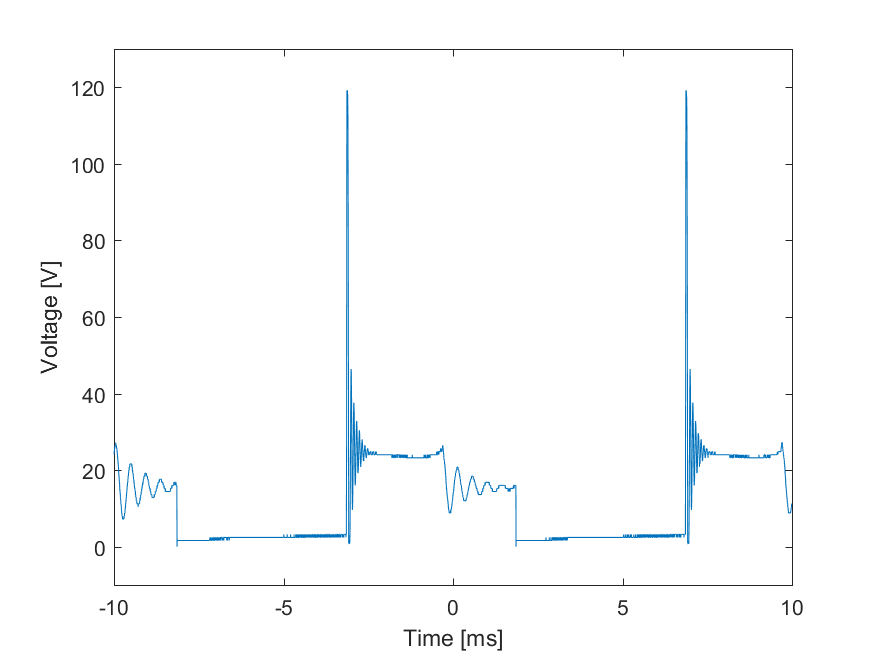
\includegraphics[width=\textwidth]{sim_raw}
    \caption{Engine ignition system}
    \label{fig:sim_raw}
\end{figure}

The ignition simulator works much the same way as the actual ignition system on a gasoline engine. It uses an ignition coil, condenser, and spark plug from a car engine. Instead of points, it has a transistor controlled by a function generator to simulate any desired engine RPM. As seen in the Figure above, the output from the simulator is very similar to that measured on the gasoline engine. The simulator allowed design and testing of the ignition signal generator to be performed in a lab without a running engine.


\subsection{Specifications}
With the ignition signal simulator, the tachometer's primary function could be tested. Using the signal generated by the simulated ignition as an input allowed the response of the gauge to be observed. The power supply, tachometer operation, and deliverability specifications are discussed in their own sections in further detail.

The engine sensor input operation was confirmed by simulating the engine sensors with a potentiometer circuit. A calibration routine is in place such that the tachometer can be calibrated to the sensors on the power boat. The detachable display is the method for displaying the sensor's outputs.

\subsubsection{Power Supply}
The power supply was required to have an output voltage within 5\% of the specified output and less than 100mV of ripple. With the power supply constructed, both of these specifications were measured. Shown below in Figure~\ref{fig:ps_dc} is the output of the power supply, measured with DC coupling on an oscilloscope.

\begin{figure}[H]
    \centering
    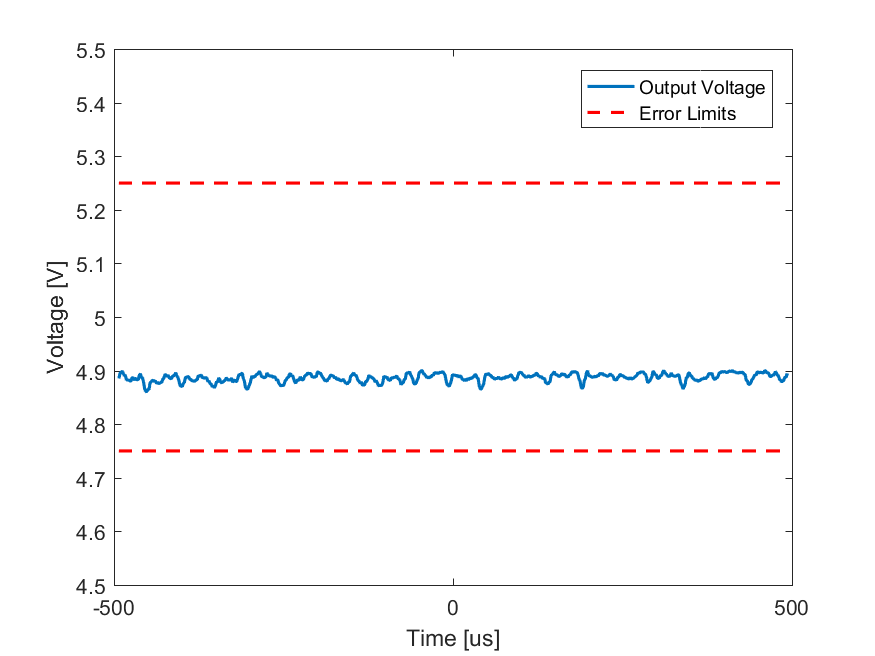
\includegraphics[width=\textwidth]{power_supply_dc}
    \caption{Power supply output, DC coupling}
    \label{fig:ps_dc}
\end{figure}

The output voltage was found to be well within the specified 5\% error region. By switching the oscilloscope to AC coupling, the output ripple was more easily measured. Shown below in Figure~\ref{fig:ps_ac} is the output ripple of the power supply.

\begin{figure}[H]
    \centering
    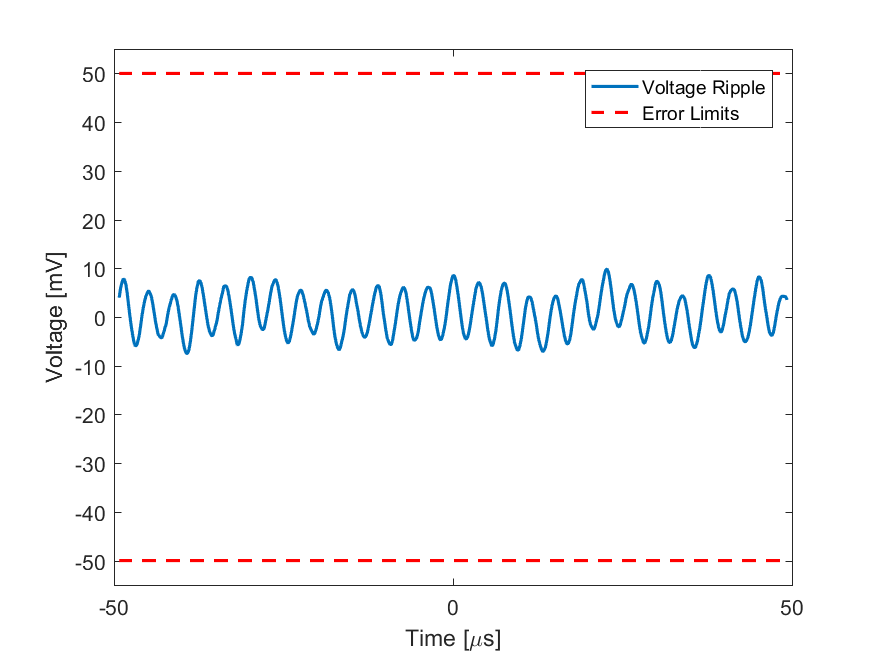
\includegraphics[width=\textwidth]{power_supply_ac}
    \caption{Power supply output, AC coupling}
    \label{fig:ps_ac}
\end{figure}

The ripple is around 20m$V_{PP}$, significantly lower than the specified 100m$V_{PP}$. Furthermore, the power supply PCB was laid out such that a total of five output capacitors could be populated, however only two were needed to achieve this result. If lower ripple was desired, more capacitors could be added to further improve the power supply's performance.

\subsubsection{Tachometer Operation}
Tachometer operation was verified in two separate ways: first with the ignition signal simulation, and second by connecting it to a car with a four cylinder engine. These tests showed that the tachometer and power supply were capable of operating with the presence of the ignition and other electrical system noise from the vehicle. The accuracy of the tachometer output was measured by comparing the gauge and LCD output values against known input values, results are shown in Figure~\ref{fig:rpm}.

\begin{figure}[H]
    \centering
    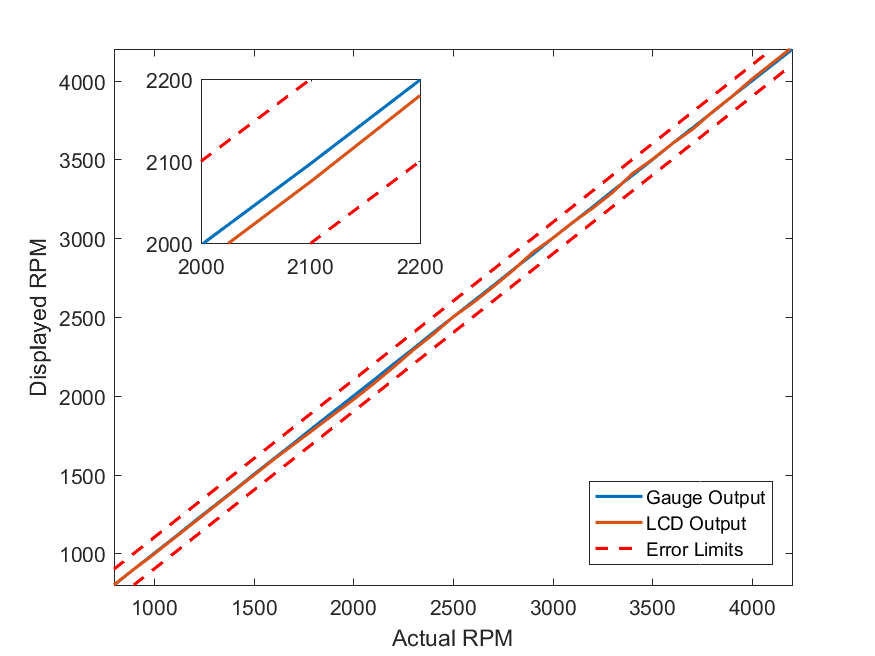
\includegraphics[width=\textwidth]{rpm}
    \caption{Gauge and LCD output accuracy}
    \label{fig:rpm}
\end{figure}

The plot shows both the LCD and gauge were within the $\pm$100 RPM error limits, with little variation between the two outputs. Furthermore, the tests revealed that under typical operation, the gauge and LCD outputs are within 10 RPM of the measured value.

\subsubsection{Deliverability}
As specified, the tachometer is deliverable to the customer with a box and secure mounting hardware protect the PCB and internal components. Proper mounting, connectors, and cable relief ensure long life of the tachometer. 

Additionally, Appendix~\ref{app:user} includes documentation on the installation and use of the tachometer. The documentation is useful for the owner of the product or service technician to diagnose problems or perform a new installation.

Since the tachometer is designed to work with any engine, not just that of the 1988 Celebrity Champion, it features user calibration. Since all tachometer gauges and all engine sensors are slightly different, the tachometer must be calibrated on a per-installation basis. Calibration is done via a serial connection and features a simple, intuitive interface for calibrating the range of the tachometer gauge and the range of the analog engine sensors. As discussed in a previous section, the tachometer was tested for proper operation in a car. This proves that the tachometer can be calibrated to work in various installation environments.

Additionally, while the contract specifies that a DC-DC converter is to be built and there are to be other engine sensor inputs, the customer is mainly interested in reliable tachometer operation. Since off-the-shelf DC-DC components are often more reliable than custom power supplies, the tachometer is designed such that a linear (or switching linear replacement) could replace the power supply designed to meet contract specifications. The sensor inputs are also constructed on a different PCB, such that they do not take up additional space, or draw additional power if the customer chooses not to use them.



\section{Conclusion}
\label{sec:con}
This report discussed the purpose and design of the Tachometer for Sheaff's Buddy's Boat. This project not only provided a solution to a failed tachometer on the Champion Celebrity power boat, it modernized the boat into the digital world. In testing, this project met or exceeded all contract specifications. Additionally, the detachable display that displayed engine oil pressure and temperature, battery voltage, and engine RPM was made to be hot swappable. With the final revision of the printed circuit board, the tachometer functioned as desired and was delivered to the customer.

\newpage
\bibliography{references}
\bibliographystyle{ieeetr}
\newpage

\appendix
\renewcommand\pagenumbering[1]{}
\section{Project Contract}
\label{app:contract}
\begin{singlespacing}
\begin{center}
\LARGE{Tachometer Contract}\\
\vspace{1.3em}
\large{Colin Leary, EE}\hfill\\
\large{Chris Martin, CE}\\
\vspace{1.3em}
\large{\today}

\end{center}


\subsection*{Summary}
A tachometer is to be built which will be capable of driving an analog tachometer gauge. The specified project has a DC-DC converter that converts nominal 12V to 3.3V $\pm5\%$ to run the microcontroller and other components. The tachometer shall be constructed on a PCB and can not utilize a development board. The gauge will be accurate to 100RPM between 1000RPM and 4000RPM. The specification makes the gauge most accurate in a typical operating range.

\subsection*{Inputs \& Outputs}
\begin{itemize}
    \item RPM signal
    \item Other sensor signals
    \item Tachometer gauge
    \item Detachable display
\end{itemize}


\subsection*{Specifications}
\begin{itemize}
    \item DC-DC converter to step down nominal 12VDC to 3.3VDC $\pm$5\%, less than 100mV ripple at 500mA
    \item Able to position analog gauge needle within  100RPM between 1000RPM and 4000RPM
    \item Built on printed circuit board and no development board
    \item Deliverable product to customer
    \item Capable of showing RPM, coolant temperature, oil pressure, and battery voltage
\end{itemize}
    \pagenumbering{gobble} % Turn off page numbering for titles and tables

\begin{table}[H]
\centering

\label{my-label}
\begin{tabular}{lllllll}
            &  &                          &  &              &  &                          \\ \cline{1-3} \cline{5-7} 
Colin Leary & ~~~~~~~~~~~~~~~~~ & \multicolumn{1}{r}{Date} & ~~~~~~~~~~~~~~~ & Chris Martin & ~~~~~~~~~~~~~~~~~ & \multicolumn{1}{r}{Date}
\end{tabular}
\end{table}

\end{singlespacing}


\section{Tachometer Schematic}
\label{app:schem}
\begin{figure}[H]
    \centering
    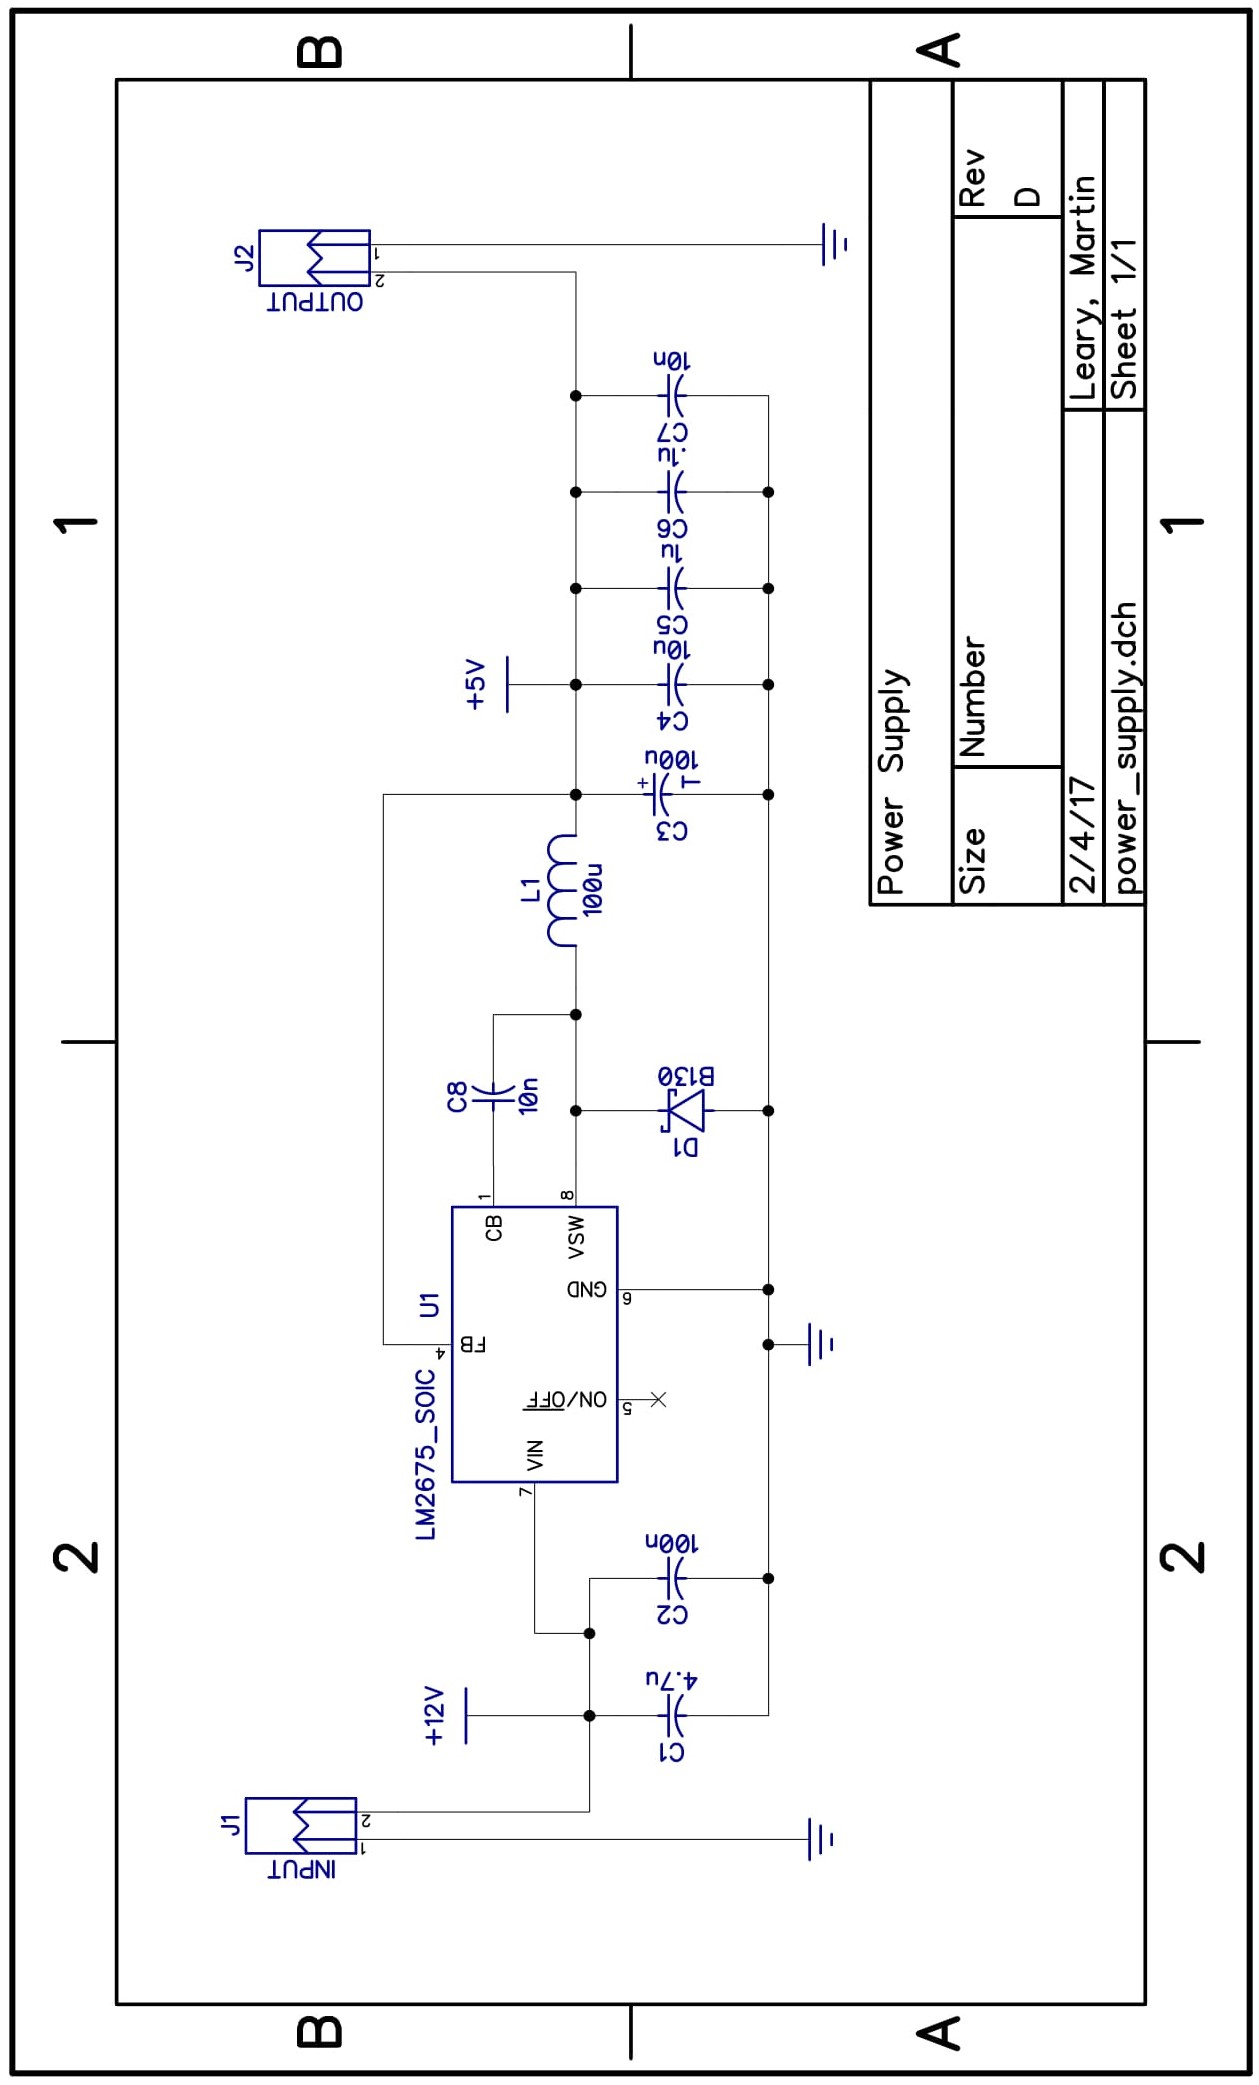
\includegraphics[width=.8\textwidth]{documents/ps_schem}
\end{figure}

\begin{figure}[H]
    \centering
    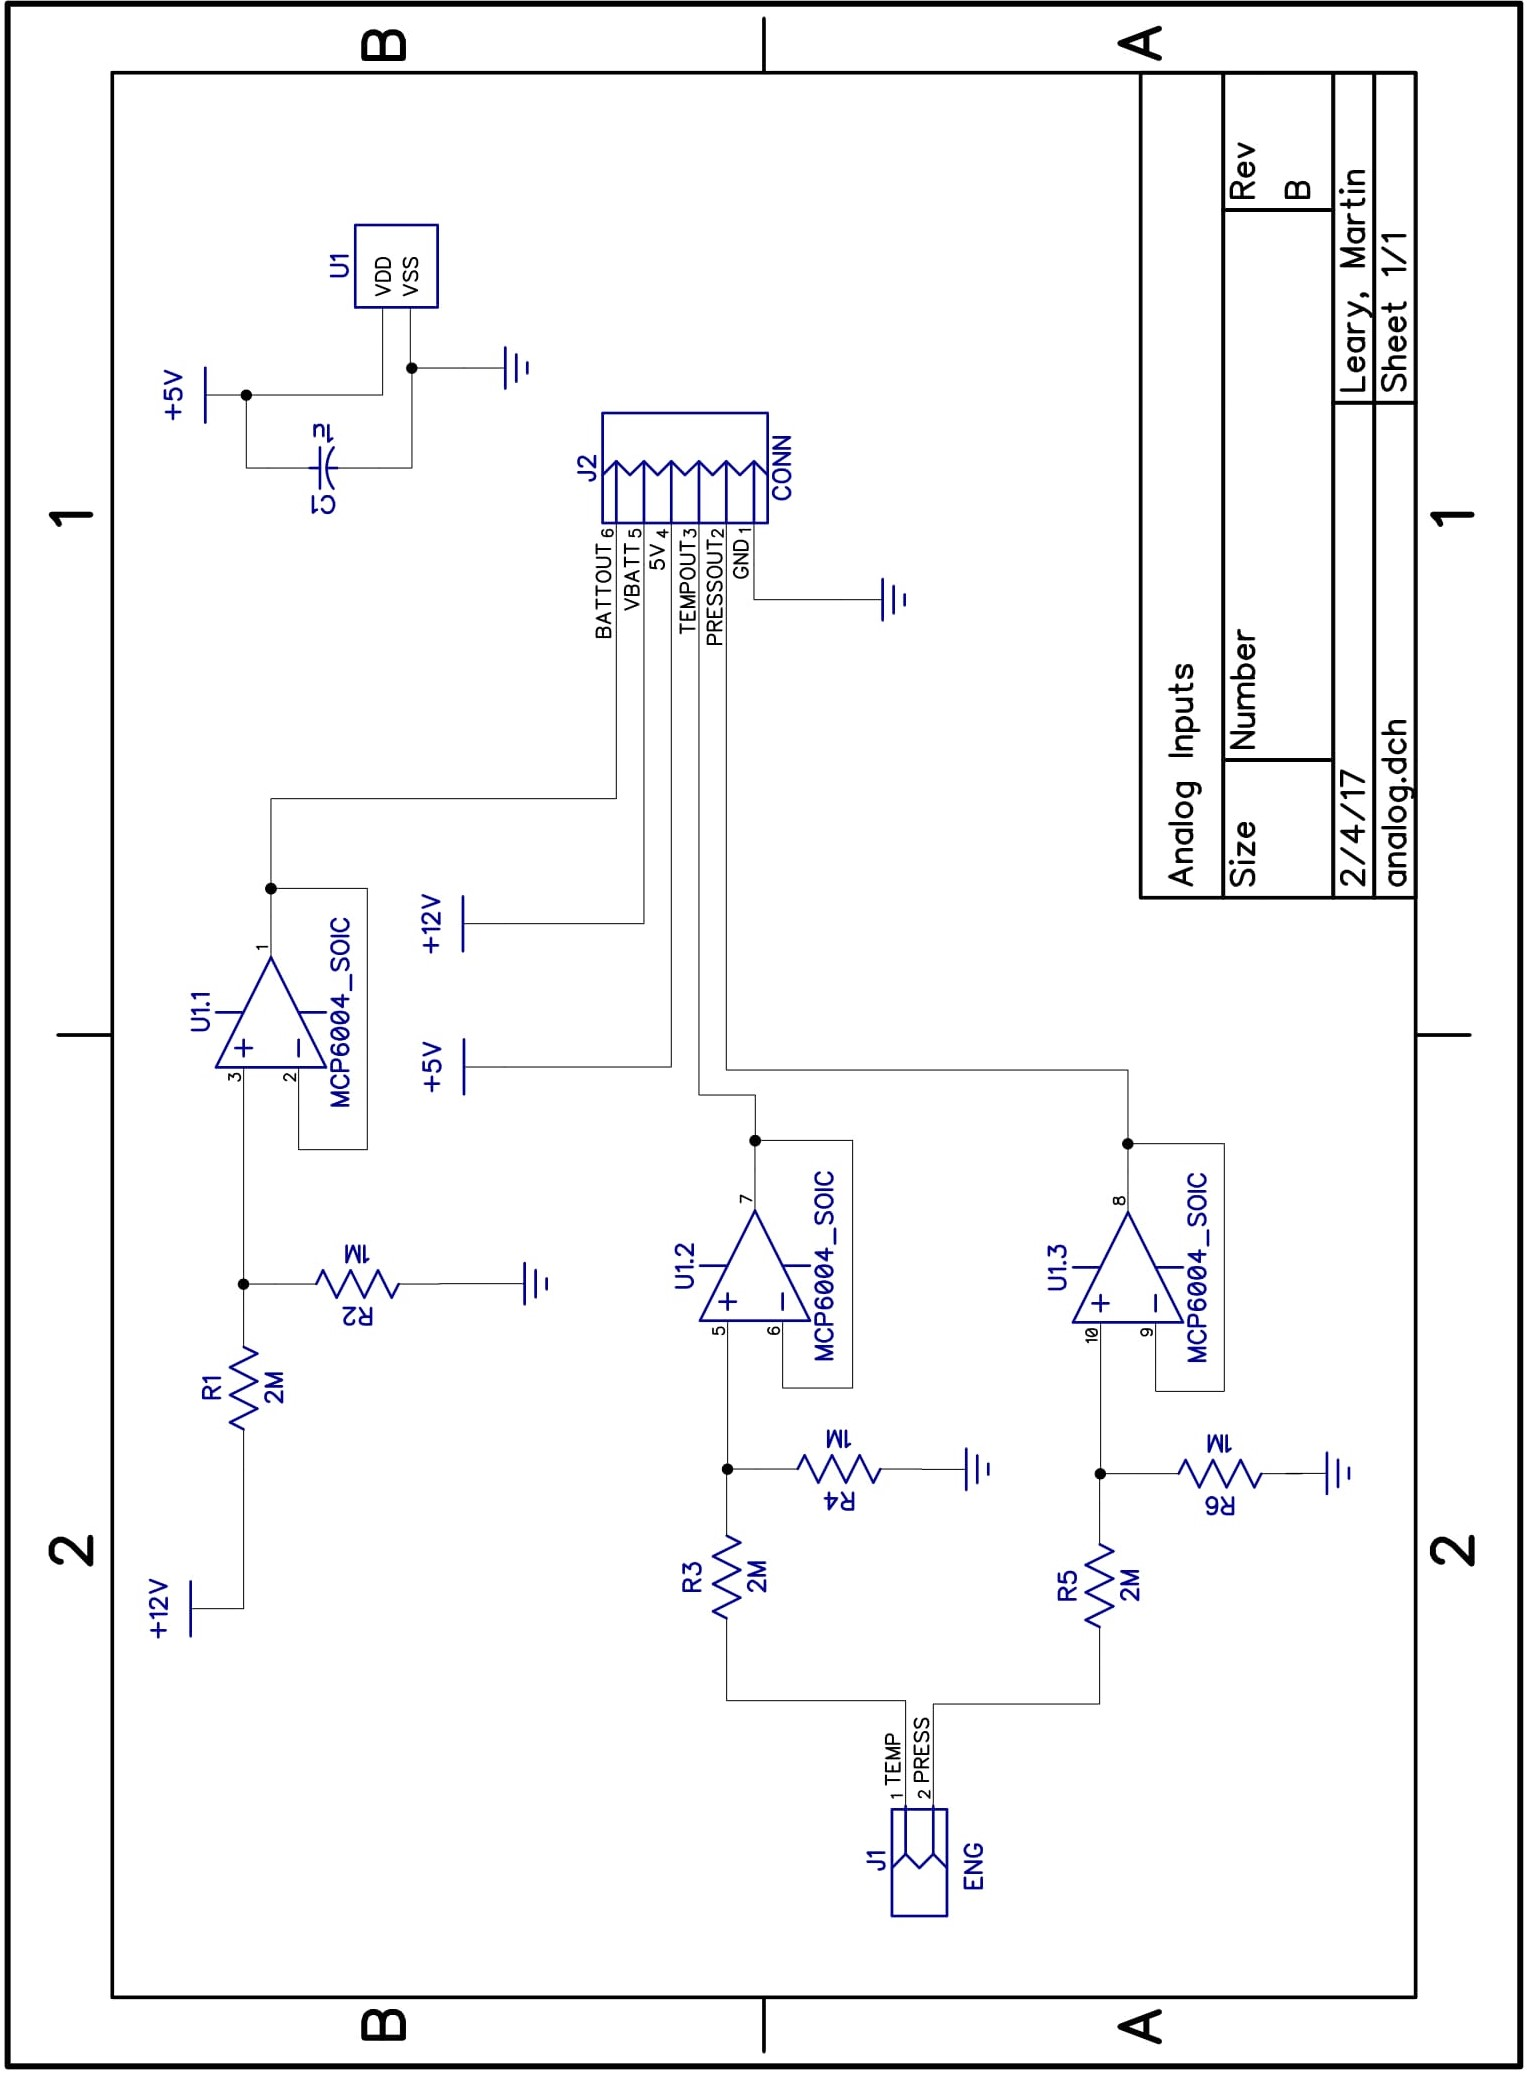
\includegraphics[width=\textwidth]{documents/analog_schem}
\end{figure}

\begin{figure}[H]
    \centering
    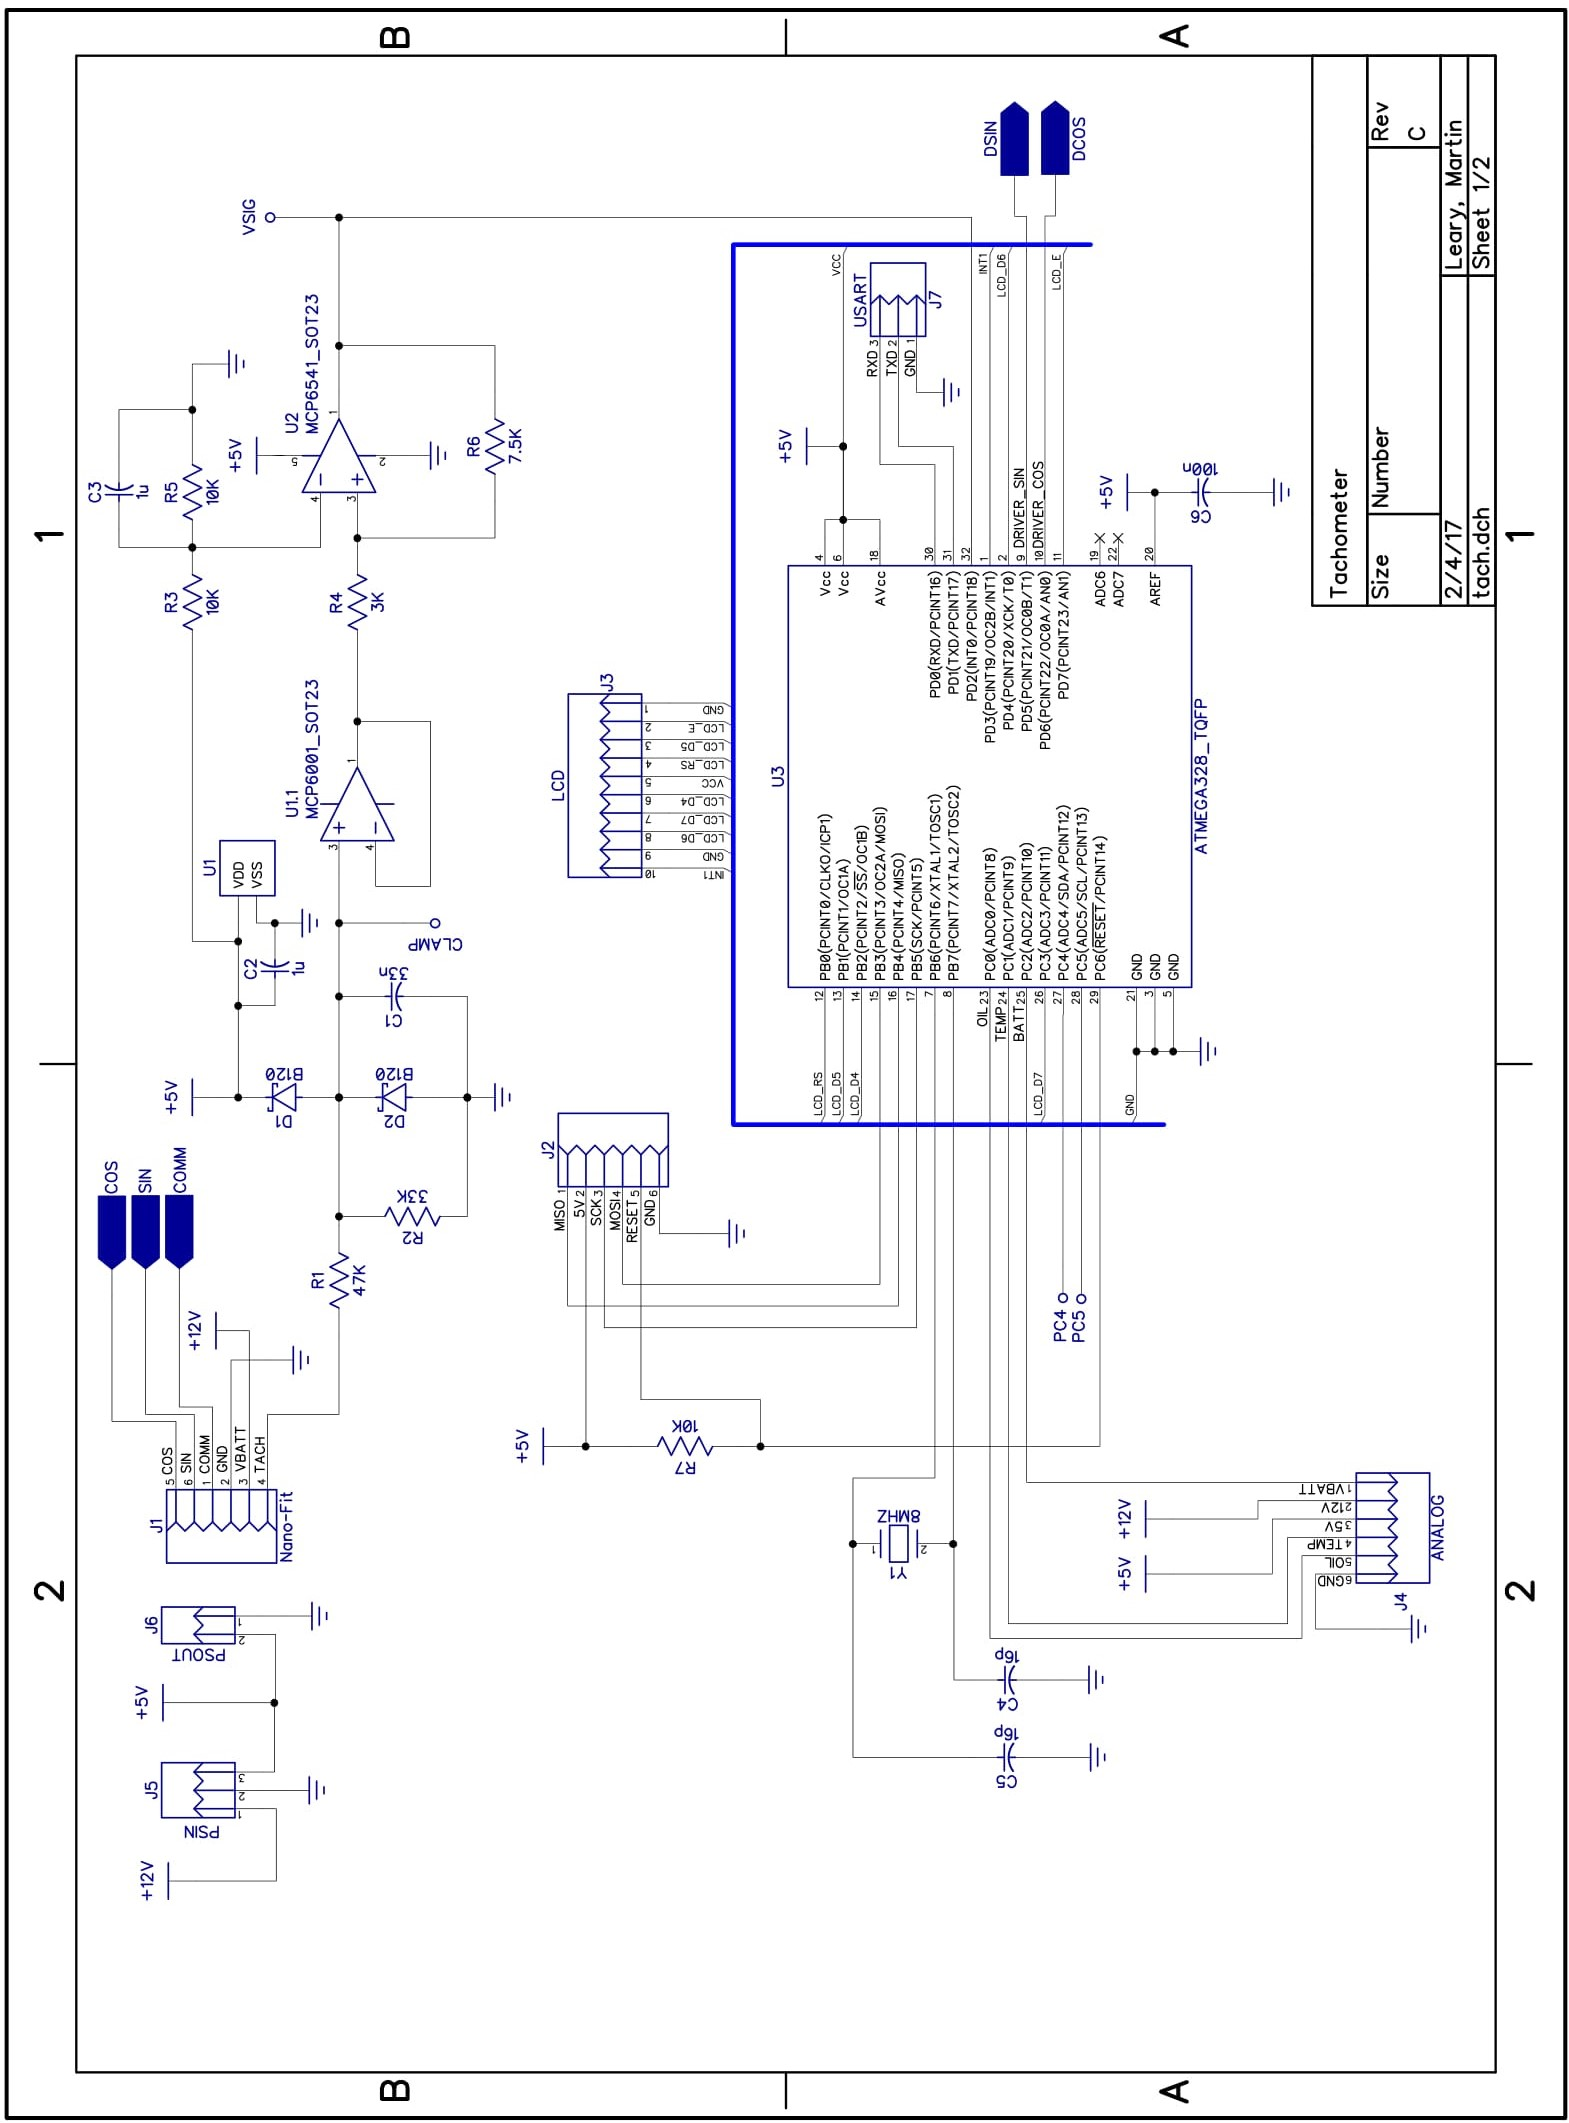
\includegraphics[width=\textwidth]{documents/tach_schem1}
\end{figure}

\begin{figure}[H]
    \centering
    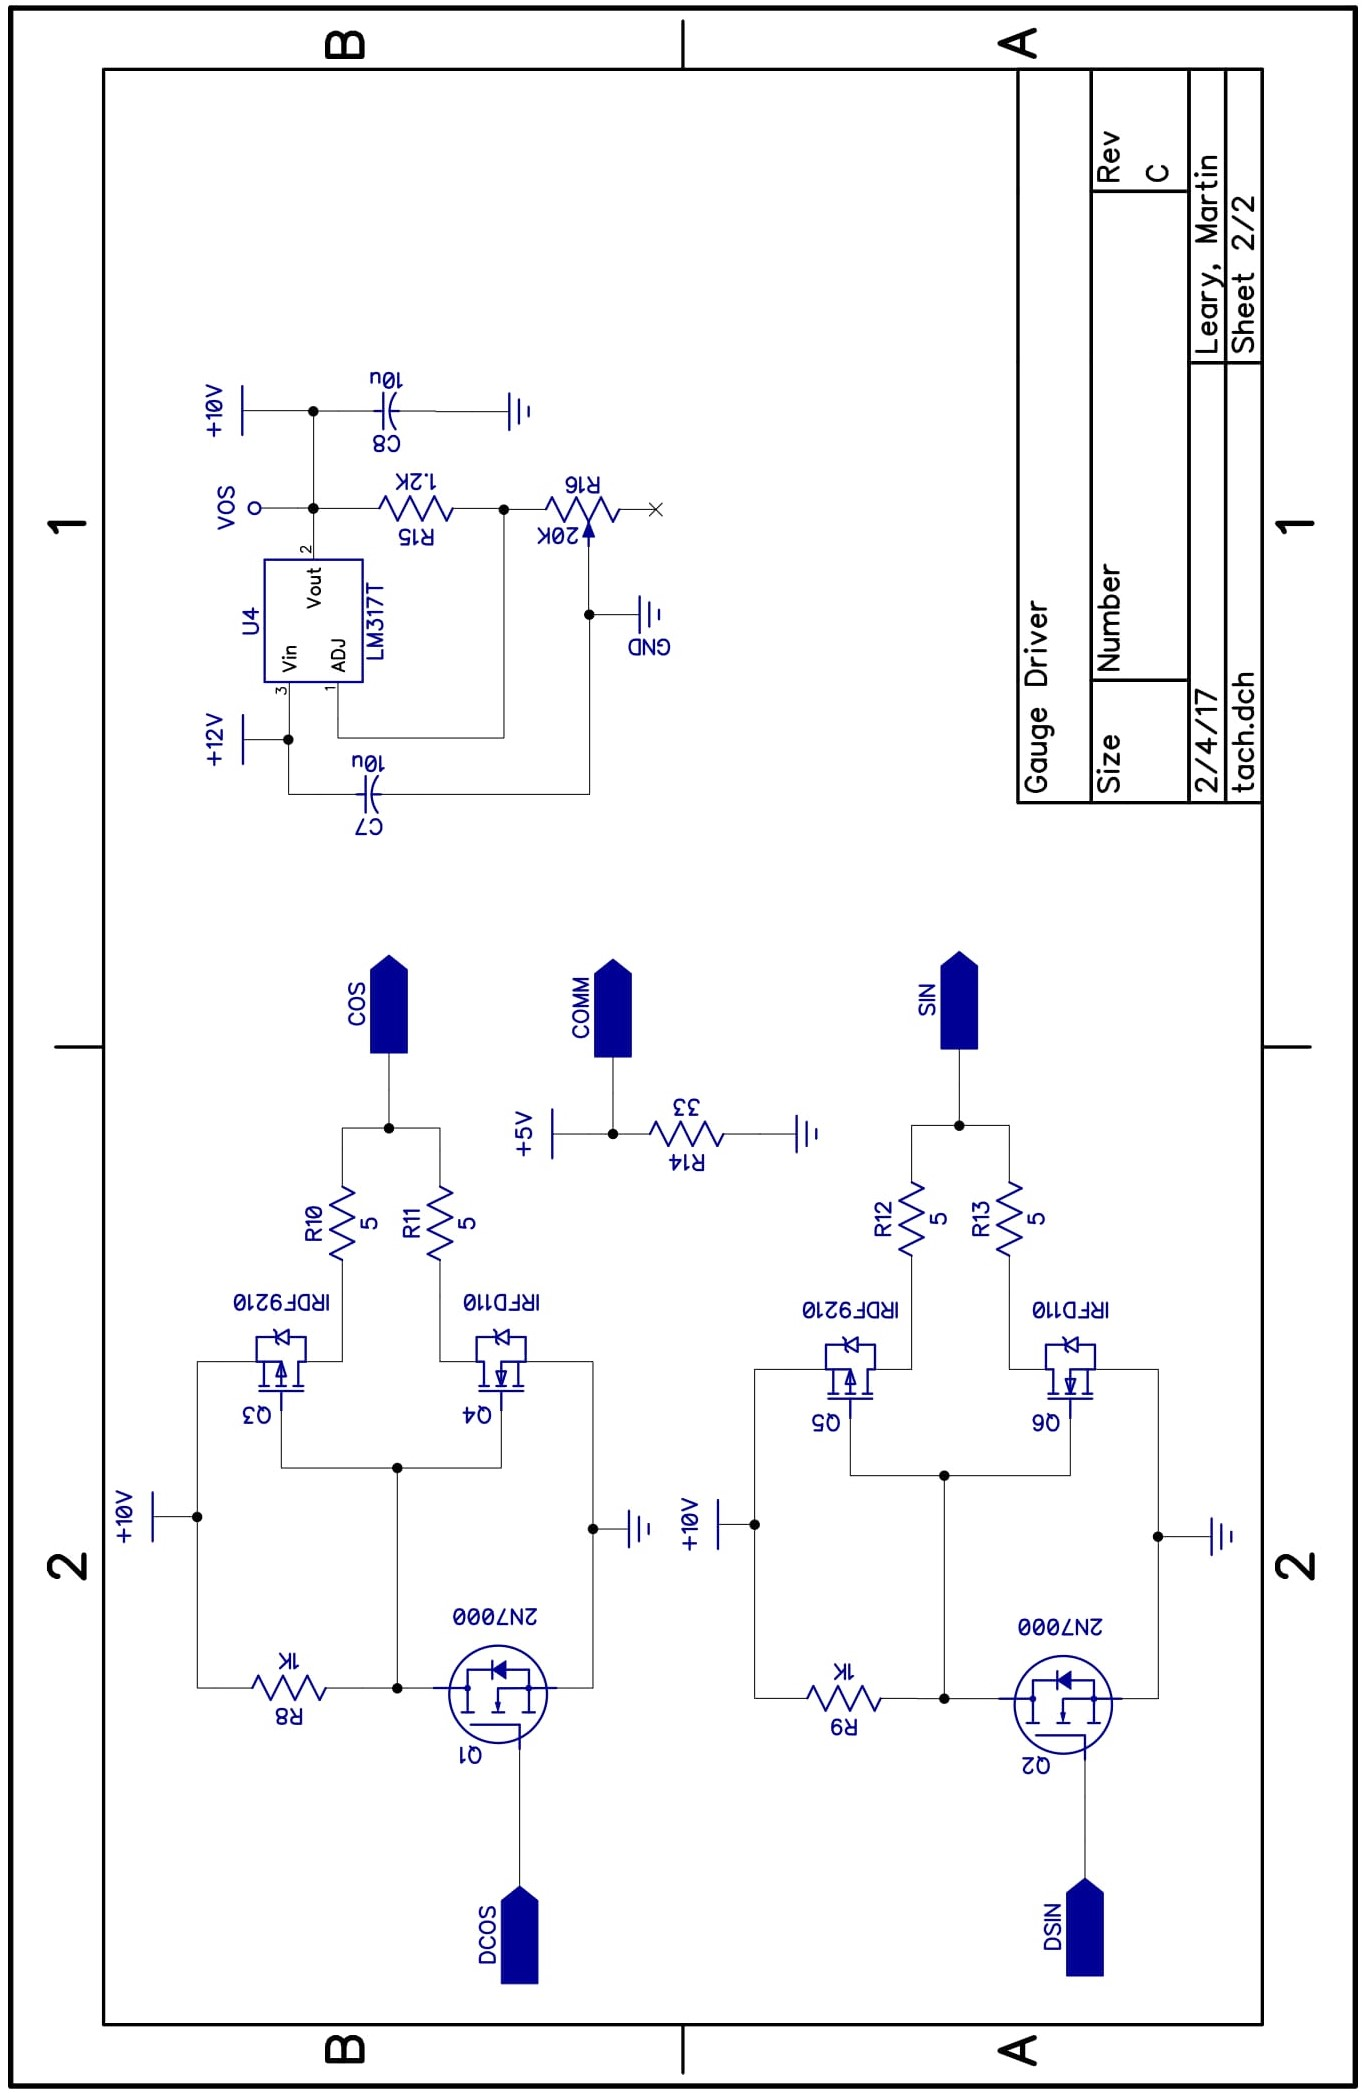
\includegraphics[width=.95\textwidth]{documents/tach_schem2}
\end{figure}

\newpage\clearpage
\section{Parts List}
\label{app:parts}
\begin{figure}[H]
    \centering
    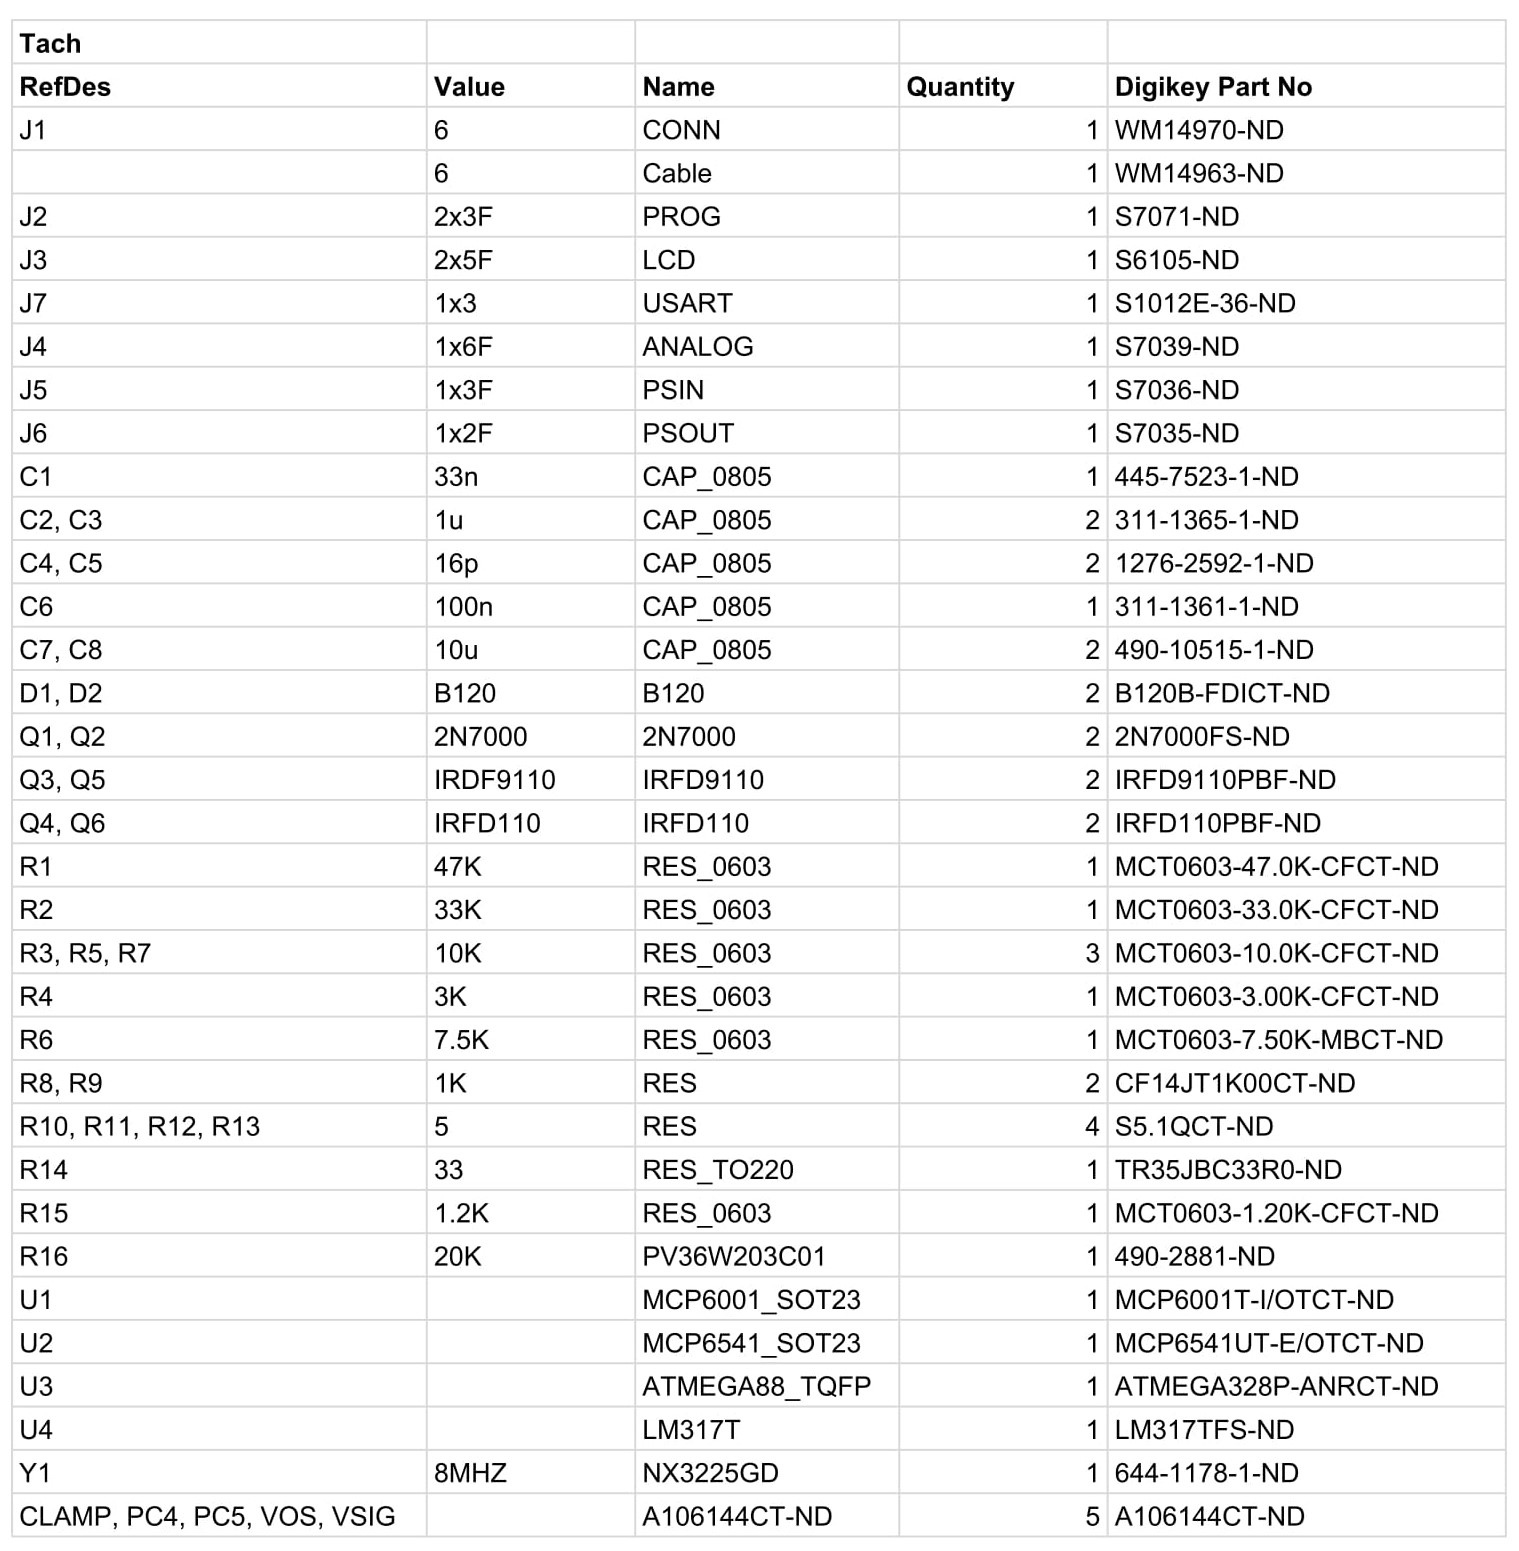
\includegraphics[width=\textwidth]{documents/bom_1}
\end{figure}

\begin{figure}[H]
    \centering
    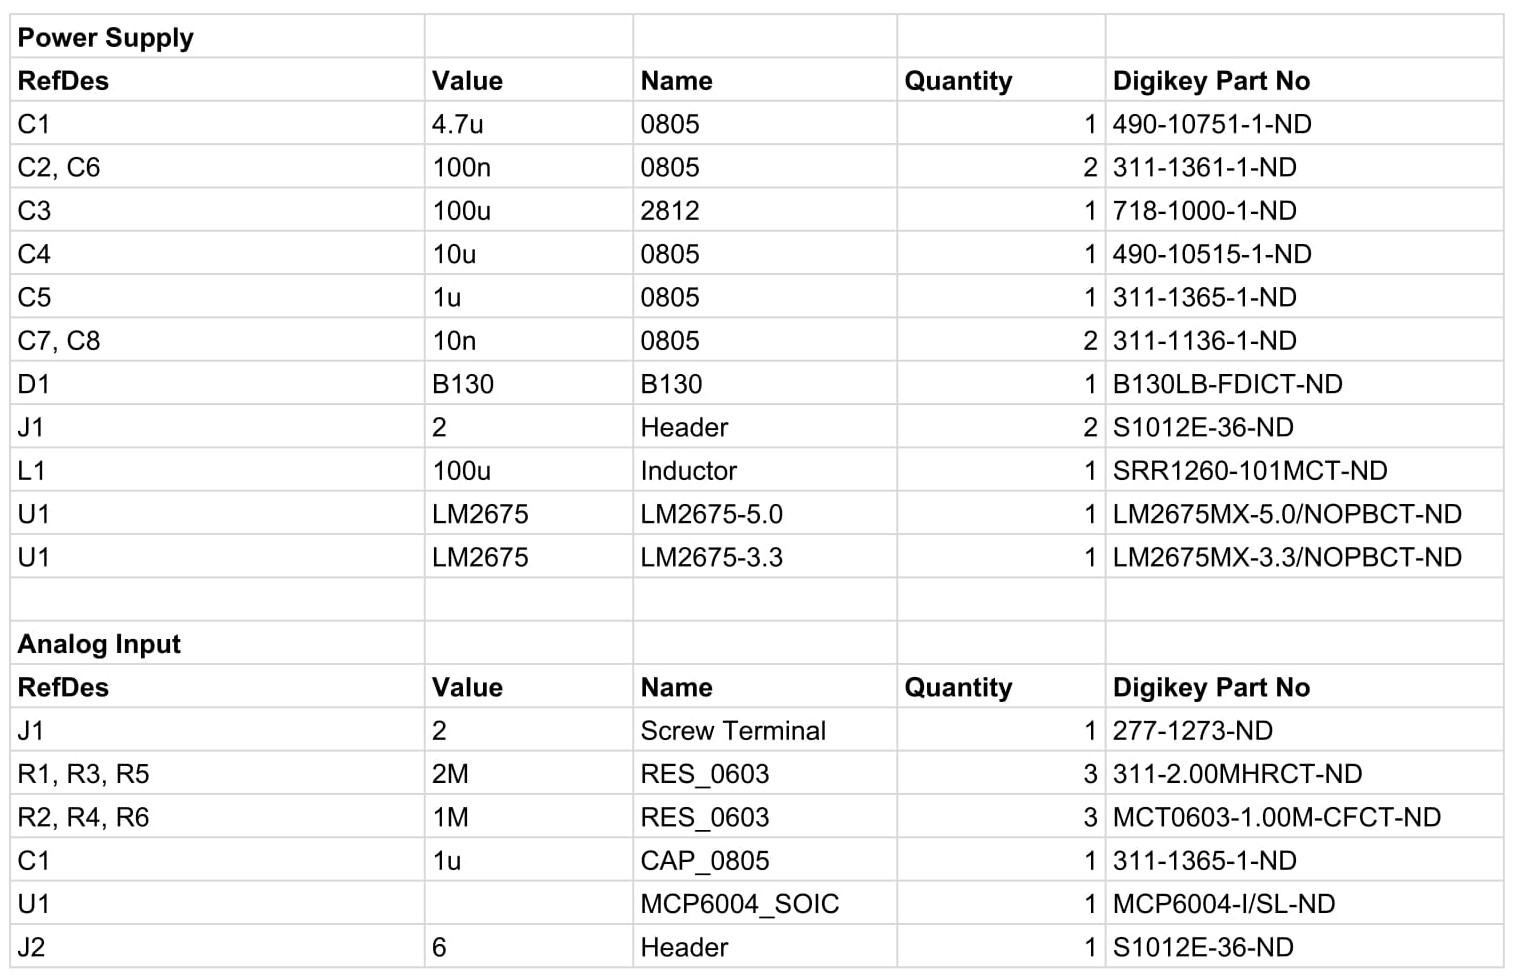
\includegraphics[width=\textwidth]{documents/bom_2}
\end{figure}

\newpage\clearpage
\section{User Documentation}
\label{app:user}



%\section{Overview}
{\large\textbf{1~~~~Overview}}

The tachometer is intended to interface seamlessly with a 1988 Celebrity Champion power boat. Its primary function is to determine the engine revolutions per minute (RPM) and drive the appropriate gauge to display that RPM. The tachometer is also capable of additional functionality, such as having an LCD screen attached, measuring and displaying oil temperature, coolant temperature, and battery voltage. Additional equipment and documentation is required to enable these additional features.

The tachometer, shown in Figure~\ref{fig:mamad}, is broken into several input/output blocks. Table~\ref{tab:descd} gives information about the labelled portions of Figure~\ref{fig:mamad}.
\begin{figure}[H]
    \centering
    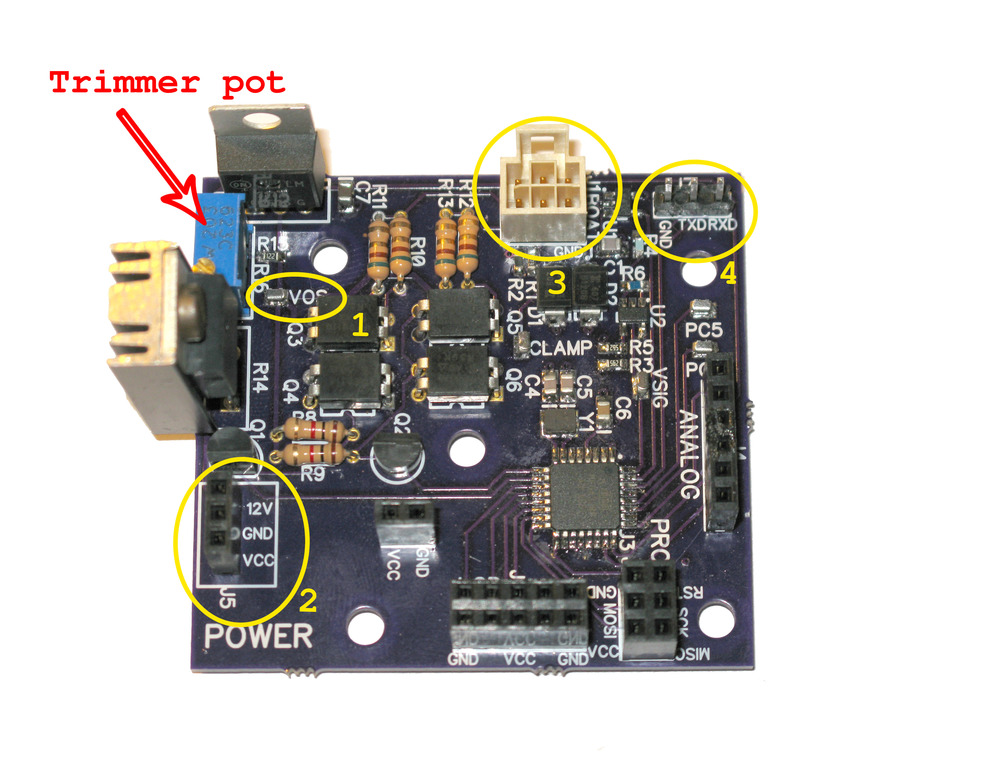
\includegraphics[width=.9\textwidth]{documents/mamaboard}
    \caption{Tachometer}
    \label{fig:mamad}
\end{figure}

% Please add the following required packages to your document preamble:
% \usepackage{booktabs}
\begin{table}[H]
\centering
\caption{Connector descriptions}
\label{tab:descd}
\begin{tabular}{@{}cl@{}}
\toprule
\textbf{Connection} & \textbf{Description} \\ \midrule
1 & Test point for 10V power supply \\
2 & Connector for 5V power supply \\
3 & Connector to boat system \\
4 & Connector for tachometer calibration \\ \bottomrule
\end{tabular}
\end{table}



%\section{Installation}
{\large\textbf{2~~~~Installation}}

Connection~3 is used for interfacing the tachometer to the electrical system on a boat. Figure~\ref{fig:boatcond} shows the pinout.

\begin{figure}[H]
    \centering
    \includegraphics[width=.4\textwidth]{documents/connector}
    \caption{Pinout of Connector 3}
    \label{fig:boatcond}
\end{figure}

The 12V and GND pin connect to the nominal 12V electrical system of a boat and the IGN pin connects to the ignition signal from a gasoline engine. The SIN, COS, and COMM pins connect to the sine, cosine, and common pins of a three-wire  tachometer gauge.

%\section{Calibration}
{\large\textbf{3~~~~Calibration}}

First, the  gauge drive voltage must be set. This can be done by adjusting the trimmer pot shown in Figure~\ref{fig:mamad} until the voltage read at Connection~1 is 10V.

Next, the  gauge operating range and direction must be set, this is done by connecting a 5V logic serial adapter to Connection~4. The tachometer communicates using RS232 at 9600 baud with 8-bit words and one stop bit. After connecting the serial adapter and powering on the tachometer, type CTRL+C on the computer keyboard in a serial console to enter configuration mode. Choose menu option number one, Calibrate tachometer range, to configure the operating range. Press and hold the 1 key until the tachometer needle is at 1000 RPM. The needle should rotate clockwise, if it rotates anti-clockwise, swap the SIN and COS pins on Connector~3. After setting the gauge to 1000 RPM, press enter and hold the 1 key again until the tachometer is at 2000 RPM. Then press enter again to complete calibration.

Menu option two tests the tachometer to confirm a successful calibration without the need to run the engine.

When calibration is done, press the escape key to save the calibration data. The tachometer is ready for use.

%\section{Power Supply}
{\large\textbf{4~~~~Power Supply}}

If the tachometer is not functioning properly, the first thing to check are the power supplies. There are two power supplies on the tachometer, a 10V supply to control the gauge driver circuitry, and a 5V supply for the microcontroller. The 10V supply has a designated test point, Connection 1, labelled \verb|VOS|. If the voltage at \verb|VOS| is not 10V $\pm$100mV, the  trimmer pot can be used to adjust the voltage. If the voltage can not be adjusted to the specified range, the voltage regulator, labelled \verb|U4|, may need replacement. The regulator is an LM317T.

The second power supply attaches to Connection~2. The connector, \verb|J6|, has two pins, a 0V reference and a  5V pin. If the voltage measured across these pins is not 5V, then the power supply may need replacement. A power supply was designed specifically for this project, and may be installed on top tachometer. However, the tachometer is designed such that an off-the-shelf DC-DC converter could be installed should the original fail.

There are many options of DC-DC converter that will work, however it must follow the pinout (shown on main board), and must fit in the provided space. A switching regulator such as the Murata OKI-78SR-5/1.5-W36-C is recommended, though a simple linear regulator such as an LM7805 will also work. If a linear regulator is used, a heat will be required.


\end{document}